\documentclass[UTF8,a4paper,12pt]{ctexbook} %ctex-  ctexart
 \usepackage{graphicx}%学习插入图
 \usepackage{verbatim}%学习注释多行
 \usepackage{booktabs}%表格
 \usepackage{geometry}%图片
 \usepackage{amsmath} 
 \usepackage{amssymb}
 \usepackage{listings}%代码
 \usepackage{color}
 \usepackage{xcolor}
 \usepackage{enumitem}%列表格式
 \usepackage{hyperref}
 \usepackage{url}
 
 
 \graphicspath{{figure/}}
 \CTEXsetup[format+={\flushleft}]{section}
 
  %代码效果定义
  \definecolor{mygreen}{rgb}{0,0.6,0}
  \definecolor{mygray}{rgb}{0.5,0.5,0.5}
  \definecolor{mymauve}{rgb}{0.58,0,0.82}
  \lstset{ %
  	backgroundcolor=\color{white},   % choose the background color
  	basicstyle=\footnotesize\ttfamily,        % size of fonts used for the code
  	columns=fullflexible,
  	breaklines=true,                 % automatic line breaking only at whitespace
  	captionpos=b,                    % sets the caption-position to bottom
  	tabsize=4,
  	commentstyle=\color{mygreen},    % comment style
  	escapeinside={\%*}{*)},          % if you want to add LaTeX within your code
  	keywordstyle=\color{blue},       % keyword style
  	stringstyle=\color{mymauve}\ttfamily,     % string literal style
  	frame=single,					%tb top and bottom; L left double line
  	xleftmargin=.06\textwidth, 
  	%xrightmargin=.1\textwidth,
  	rulesepcolor=\color{red!20!green!20!blue!20},
  	% identifierstyle=\color{red},
  	language=c++,
  }
%设置目录显示级别
\setcounter{tocdepth}{4}
\geometry{left=1.6cm,right=1.8cm,top=2cm,bottom=1.7cm} %设置文章宽度
%设置页面布局
\pagestyle{plain}
\author{\kaishu 郑华}
\title{\textbf{C++\_Basic 总结}}

 %正文排版开始
\begin{document} 
	
	\maketitle
	\tableofcontents 
		
\chapter{C++11 新特性必学}
	\section{右值操作}
		\subsection{右值 与 左值}
		\begin{itemize}
			\item \textbf{左值}: 左值是一个可以用来存储数据的变量,\textbf{有实际的内存地址},表达式结束后依然存在。她因在赋值操作符左边而得名。
			
			\item \textbf{右值}: 更准确的应该叫非左值,是一个\textbf{匿名的} \underline{临时变量},她在表达式结束时生命周期终止,不能存放数据,可以被修改,也可以不被修改(若被const 标识)
		\end{itemize}	
		
		根据这个解释,鉴别左值和右值最简单的方法是:左值可以用取地址符号“\&” 获取地址,而右值无法使用'\&'(会编译错误).
		\begin{lstlisting}
	int    x = 0;      //对象实例,有名,x 为左值
	int*   p = &++x;   //可以取地址,++x 是左值
	++x      = 10;	   //前置++ 返回的是左值,可以赋值
	p        = &x++;   //后置++ 返回一个临时对象,不能取地址或赋值,是右值,编译错误
		\end{lstlisting}
		
		因为右值是临时的,生命周期即将结束,之后无人关心他的值,所以我们\textit{可以把他的所有内容转移到其他对象中},\textbf{从而完全消除高昂的拷贝代价}。
		
		\subsection{右值引用}
			\subparagraph{表示:}
			有了右值的概念,右值引用应运而生。 C++ \textbf{使用T\&\&表示右值引用},而原来的T\&表示左值引用,分别引用右值对象和左值对象。
			
			\subparagraph{核心:}
			对一个对象使用右值引用,意味着显式的标记这个对象为右值,\textit{可以被转移来优化}。同时也相当于\textbf{为他添加了一个“临时的名字”,生命周期得到了延长},不会在表达式结束时消失,而是\textbf{与右值引用绑定在一起}。
			
				其实就是\textbf{存储临时对象的地址}。
			
			\subparagraph{右值引用绑定的对象}  返回非引用类型的函数,产生右值的表达式(算术表达式、关系表达式、位、后置递增递减)
			
			\subparagraph{生命周期}\verb|int && num = 8; //右值引用| 
			
			正常情况下,右值”8“在表达式语句结束后,其生命也就终结了(通常我们也称其具有表达式生命期),\textbf{而通过右值引用的声明,该右值又“重获新生”,}\textit{其生命期将与右值引用类型变量num的生命期一样}。只要num还“活着”,该右值临时量将会一直“存活”下去。
			
			\subparagraph{示例}:
			\begin{lstlisting}
	int&		r1 = ++x;	//左值引用
	int&&		r2 = x++;	//右值引用,引用了自增后的临时对象 Xvalue
	const int&	r3 = x++;	//常量左值引用
	const int&&	r4 = x++;	//常量右值引用,不能修改,不能转移,无实际意义
	cout << r2 << endl;			//右引用延长生命期,右值对象在表达式结束后仍然存在
			\end{lstlisting}	
			\url{https://github.com/ctzhenghua/C-NetworkPractice-Code/blob/Dev/C%2B%2B/Basic/RightValue/RightReference.cc}
			
		
		\subsection{Move 语义}
			\subsubsection{简介}	
				\verb|move|是将对象的状态或者所有权从一个对象转移到另一个对象,只是转移,没有内存的搬迁或者内存拷贝,如图所示是深拷贝和\verb|move|的区别
				
				\begin{figure}[h]
					\centering
					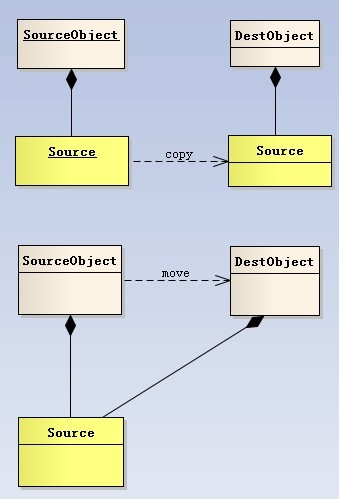
\includegraphics[angle=0,width=8cm,height=7cm]{moveANDcopy.jpg}%就在前面括号中写图片名
					\caption{UML图}
					\label{fig:winClass}
				\end{figure}
				
				\begin{lstlisting}
	//执行深拷贝
	String(const String& rhs): data_(new char[rhs.size() + 1])
	{
		strcpy(data_, rhs.c_str());
	}
				\end{lstlisting}
				这里进行了内存分配和拷贝数据.
				
				如果\verb|rhs|是个\textbf{临时对象},要是能将rhs的数据“move”到\verb|data_|中岂不是提高了运行效率,这样子你即不需要为\verb|data_|重新分配内存,又不需要去释放\verb|rhs|的内存,简直两全其美。
	
				\begin{lstlisting}
	String(String&& rhs): data_(rhs.data_)
	{
		rhs.data_ = nullptr;
	}
				\end{lstlisting}	
				
				在 c++11,一个\verb|std::vector|的 “\verb|move| 构造函数” 对某个\verb|vector|的右值引用可以单纯地从右值复制其内部 \verb|C-style| 数组的指针到新的 \verb|vector|,然后留下空的右值。这个操作不需要数组的复制,而且空的临时对象的析构也不会摧毁内存。如果\verb|vector|没有 \verb|move| 构造函数,那么复制构造函数将被调用,这时进行深拷贝。
						
				细节对比如下:
				\begin{lstlisting}
					
	//////////////////////////////拷贝构造/////////////////////////////
	class ArrayWrapper
	{
	public:
		ArrayWrapper (int n): _p_vals( new int[ n ] ), _size( n ){}
		// copy constructor
		ArrayWrapper (const ArrayWrapper& other): _p_vals( new int[ other._size  ] ), _size( other._size )
		{
				for ( int i = 0; i < _size; ++i )
				{
					_p_vals[ i ] = other._p_vals[ i ];
				}
		}
		~ArrayWrapper ()
		{
			delete [] _p_vals;
		}
	private:
		int *_p_vals;
		int _size;
	};
					
					
					
	//////////////////////////////////move 构造//////////////////
	class ArrayWrapper
	{
	public:
		// default constructor produces a moderately sized array
		ArrayWrapper ()	: _p_vals( new int[ 64 ] ), _size( 64 ){}
						
		ArrayWrapper (int n): _p_vals( new int[ n ] ), _size( n ){}
						
		// move constructor
		ArrayWrapper (ArrayWrapper&& other): _p_vals( other._p_vals  ), _size( other._size )
		{
			other._p_vals = NULL;
		}
						
		//Move other
		ArrayWrapper(ArrayWrapper&& other)
		{
			std::swap(_p_vals,other._p_vals);
			std::swap(_size, other._size);
		}
						
		// 转移赋值函数
		ArrayWrapper& operator= (ArrayWrapper&& other)
		{
			std::swap(_p_vals,other._p_vals);
			std::swap(_size, other._size);
			return *this;
		}
						
		// copy constructor
		ArrayWrapper (const ArrayWrapper& other): _p_vals( new int[ other._size  ] ), _size( other._size )
		{
			for ( int i = 0; i < _size; ++i )
			{
				_p_vals[ i ] = other._p_vals[ i ];
			}
		}
		~ArrayWrapper ()
		{
			delete [] _p_vals;
		}
		
	private:
		int *_p_vals;
		int _size;
	};				
				\end{lstlisting}
			\subsubsection{使用场景}
				\begin{enumerate}
					\item C++ 标准库使用比如\verb|vector::push_back |等这类函数时,会对参数的对象进行复制,连数据也会复制.这就会造成对象内存的额外创建, 本来原意是想把参数\verb|push_back|进去就行了.
					\item \verb|C++11| 提供了\verb|std::move| 函数来\textbf{把左值转换为}\verb|xrvalue|, 而且新版的\verb|push_back|也支持\verb|&&|参数的重载版本,这时候就可以高效率的使用内存了
					\item 对指针类型的标准库对象并不需要这么做.
				\end{enumerate}	
				
				\url{http://blog.csdn.net/infoworld/article/details/50736633}
				\begin{lstlisting}
	void TestSTLObject()
	{
		std::string str = "Hello";
		std::vector<std::string> v;
		
		// uses the push_back(const T&) overload, which means
		// we'll incur the cost of copying str
		v.push_back(str);
		std::cout << "After copy, str is \"" << str << "\"\n";
		
		// uses the rvalue reference push_back(T&&) overload,
		// which means no strings will be copied; instead, the contents
		// of str will be moved into the vector.  This is less
		// expensive, but also means str might now be empty.
		v.push_back(std::move(str));
		std::cout << "After move, str is \"" << str << "\"\n";
		
		std::cout << "The contents of the vector are \"" << v[0]
		<< "\", \"" << v[1] << "\"\n";	
	}
	
	/*
		After copy, str is "Hello"
		After move, str is ""
		The contents of the vector are "Hello", "Hello"
	*/
				\end{lstlisting}
				如果不用\verb|std::move|,拷贝的代价很大,性能较低。使用\verb|move|几乎没有任何代价,只是转换了资源的所有权。如果一个对象内部有较大的对内存或者动态数组时,很有必要写\verb|move|语义的拷贝构造函数和赋值函数,避免无谓的深拷贝,以提高性能。
				\begin{lstlisting}
	std::list< std::string > tokens;//省略初始化...
	std::list< std::string > t = tokens;
	
	std::list< std::string > tokens;
	std::list< std::string > t = std::move(tokens);				
				\end{lstlisting}
			\subsubsection{STL使用}
				\subparagraph{转移语义}
					C++ 标准库中的 \textbf{string、vector、deque等组件都实现了转移构造函数和转移赋值函数},可以利用转移语义优化,所以\textbf{现在在函数里返回一个大容器对象是非常有效的}。
					
					这些标准容器(除\verb|std::array|) 还特别的增加了\verb|emplace()|系列函数,可以使用转移语义直接插入元素,进一步提高运行效能。
			\begin{lstlisting}
	vector<complex<double>> v;	//标准序列容器
	v.emplace_back(3,4);        //直接使用右值插入元素,无须构造再拷贝

	map<string, string>m;
	m.emplace("metroid","prime");//直接使用右值插入元素,无须构造再拷贝
	m.push_back("methroid","prime");// 这样是不行的,wrong			
			\end{lstlisting}
				\subparagraph{新容器}
					\begin{itemize}
						\item \textbf{array}:提供了定长数组容器\verb|array|,相比于普通数组更安全、更易使用。\verb|array|是定长数组,所以不支持诸如插入、删除等改变容器大小的操作,但是可以对元素进行赋值改变其值。
						\begin{lstlisting}
	array<int, 5> c4 = {0, 1, 2, 3, 4};
	c4[3] = 100; // can't insert since the array size is fixed.
	for(auto it4_1 = c4.begin(); it4_1 != c4.end(); it4_1++)
	{
		cout<<*it4_1<<'\t';
	}
						\end{lstlisting}
						
						\item \textbf{forward\_list}:提供了一个快速的、安全的\textbf{单向链表}实现。因为是单向链表,所以也就没有\verb|rbegin、rend|一类的函数支持了。
			
						同样是因为单向链表的缘故,无法访问到给定元素的前驱,所以没有提供\verb|insert|函数,而对应提供了一个\verb|insert_after|函数,用于在给定元素之后插入节点。\verb|erase_after、emplace_after|同理。
						\begin{lstlisting}
	forward_list<int> c5 = {3, 4};
	c5.push_front(2);
	c5.push_front(1);
	auto it5_1 = c5.before_begin();
	c5.insert_after(it5_1, 0);
						\end{lstlisting}
						
						\item \textbf{无关序列容器}:引入了对\verb|map、set|等关联容器的无序版本,叫做\verb|unorderer_map/unordered_set|。
						
						无序关联容器不使用键值的比较操作来组织元素顺序,而是\textbf{使用哈希}。这样在某些元素顺序不重要的情况下,效率更高。
						\begin{lstlisting}
	unordered_map<string, int> c12;
	map<string, int> c13;
	string string_keys[5] = {"aaa", "bbb", "ccc", "ddd", "eee"};
	for(int i = 0; i < 5; i++)
	{
		c12[string_keys[i]] = i;
		c13[string_keys[i]] = i;
	}
							
	cout<<"normal map:\n";
	for(auto it13 = c13.begin(); it13 != c13.end(); it13++)
		cout<<it13->first<<':'<<it13->second<<'\t';
	cout<<endl;
							
	cout<<"unordered map:\n";
	for(auto it12 = c12.begin(); it12 != c12.end(); it12++)
		cout<<it12->first<<':'<<it12->second<<'\t';
	cout<<endl;
						\end{lstlisting}
						
						\item \textbf{tuple}:用于方便的将不同类型的值组合起来。
						
						可以通过如下方式,获取\verb|tuple|中的元素、\verb|tuple|的长度等:
						\begin{lstlisting}
	//tuple<int, string, vector<int>> c14 = {1, "tuple", {0, 1, 2, 3, 4}}; // wrong. must explicit initialize
							
	tuple<int, string, vector<int>> c14{1, "tuple", {0, 1, 2, 3, 4}};
							
	get<0>(c14) = 2;	// 赋值-修改值
	typedef decltype(c14) ctype;
	size_t sz = tuple_size<ctype>::value;
	cout<<get<0>(c14)<<'\t'<<get<1>(c14)<<'\t'<<get<2>(c14)[0]<<'\t'<<sz<<endl;
						\end{lstlisting}
						
						\item \textbf{shrink\_to\_fit}:一般可变长容器会预先多分配一部分内存出来,以备在后续增加元素时,不用每次都申请内存。所以有size和capacity之分。size是当前容器中存有元素的个数,而capacity则是在不重新申请内存的情况下,当前可存放元素的最大数目。而shrink\_to\_fit就表示将capacity中的多余部分退回,使其回到size大小。但是,这个函数的具体效果要依赖于编译器的实现
						\begin{lstlisting}
	vector<int> c11;
	for(int i = 0; i < 24; i++)
		c11.push_back(i);
								
	cout<<c11.size()<<'\t'<<c11.capacity()<<endl;
	c11.shrink_to_fit();
	cout<<c11.size()<<'\t'<<c11.capacity()<<endl;
						\end{lstlisting}
					\end{itemize}
		\subsection{完美转发}	
			右值引用类型是独立于值的,一个右值引用参数作为函数的形参,在函数内部再转发该参数的时候它已经变成一个左值,并不是他原来的类型。
			
			如果我们需要一种方法能够按照参数原来的类型转发到另一个函数,这种转发类型称为完美转发
			
			\begin{lstlisting}
	template<typename T>
	void print(T& t){
	    cout << "lvalue" << endl;
	}
	template<typename T>
	void print(T&& t){
	    cout << "rvalue" << endl;
	}
	 
	template<typename T>
	void TestForward(T && v){
	    print(v);
	    print(std::forward<T>(v));
	    print(std::move(v));
	}
	 
	int main(){
	    TestForward(1); // l r r
	    int x = 1;
	    TestForward(x); // l l r
	    TestForward(std::forward<int>(x)); // l r r
	    return 0;
	}
			\end{lstlisting}
	\section{面向对象改进}
		\subsection{override 与 final 标识符}
			我总觉得 C++中虚函数的设计很差劲,因为时至今日仍然\textbf{没有一个强制的机制来标识虚函数会在派生类里被改写}。\textbf{vitual关键字是可选的},这使得阅读代码变得很费劲。因为可能需要追溯到继承体系的源头才能确定某个方法是否是虚函数。\textbf{为了增加可读性,我总是在派生类里也写上virtual关键字},并且也鼓励大家都这么做。即使这样,仍然会产生一些微妙的错误。看下面这个例子:
			\begin{lstlisting}[language=C++]
	class A 
	{
	public:
		virtual void f(short) {std::cout << "A::f" << std::endl;}
	};
	class B : public A
	{
	public:
		virtual void f(int) {std::cout << "B::f" << std::endl;}
	};			
			\end{lstlisting}
			
			\textbf{B::f 按理应当重写 A::f}。然而二者的声明是不同的,一个参数是short,另一个是int。\textbf{因此B::f只是拥有同样名字的另一个函数(重载)而不是重写}。当你通过A类型的指针调用f()可能会期望打印出B::f,但实际上则会打出 f(short)而不是f(int) 。另一个很微妙的错误情况:参数相同,但是基类的函数是const的,派生类的函数却不是。
			\begin{lstlisting}[language= C++]
	class A 
	{
	public:
		virtual void f(int) const {std::cout << "A::f " << std::endl;}
	};
	class B : public A
	{
	public:
		virtual void f(int) {std::cout << "B::f" << std::endl;}
	};			
			\end{lstlisting}
			
			
			同样,\textbf{这两个函数是重载而不是重写}。幸运的是,现在有一种方式能描述你的意图。新标准加入了两个新的标识符(不是关键字)
			
			\textbf{override}[\underline{派生类中使用}],表示\textbf{函数必须重写基类中的虚函数},如果派生类没有重写到将编译报错。
			
			\textbf{final}[\underline{基类中使用}],表示\textbf{派生类不应当重写这个虚函数},如果派生类重写了基类的虚函数将编译报错。【在类名后使用,显示的禁止类被继承,即不能再有派生类。在虚函数后使用final,显示的禁止该函数在子类里再被重写】
			
			\begin{lstlisting}[language=C++]
	class A
	{
	public:
		virtual void f(short) { std::cout << "A::f" << std::endl; }
		virtual void g(int) final { std::cout << "A::g" << std::endl; }
	};
	class B : public A
	{
	public:
		virtual void f(short)  override  { std::cout << "B::f" << std::endl; }
		//virtual void g(int) { std::cout << "A::g" << std::endl; } // error C3248: "main::A::g":  final'func can not be "main::B::g" Rewrite: Wu fa Bei ChongXie
		virtual void g(float) { std::cout << "A::g" << std::endl; } // ChongZai
	};			
			\end{lstlisting}
		\subsection{成员初始化}
			允许\textbf{类在声明时}使用赋值或者花括号的方式\textbf{直接初始化}。无须在函数里特别指定。	
		\subsection{Defaulted}	
			\subsubsection{-引入}
				C++ 的类有\textbf{四类特殊成员函数},它们分别是:\textbf{默认构造函数}、\textbf{析构函数}、\textbf{拷贝构造函数}以及\textbf{拷贝赋值运算符}。这些类的特殊成员函数负责创建、初始化、销毁,或者拷贝类的对象。\textbf{如果程序员没有显式地为一个类定义某个特殊成员函数,而又需要用到该特殊成员函数时,则编译器会隐式的为这个类生成一个默认的特殊成员函数}。如:
					\begin{lstlisting}
	 class X{ 
	 private: 
		 int a; 
	 }; 
	 
	 X x;					
					\end{lstlisting}
					
				程序员并\textbf{没有定义类 X 的默认构造函数},\textit{但是在创建类 X 的对象 x 的时候,又需要用到类 X 的默认构造函数},此时,\textbf{编译器会隐式的为类 X 生成一个默认构造函数}。该自动生成的默认构造函数没有参数,包含一个空的函数体,即 X::X(){ }。虽然自动生成的默认构造函数仅有一个空函数体,但是它仍可用来成功创建类 X 的对象 x
				
				但是,\textbf{如果}程序员\textbf{为类 X 显式的自定义了非默认构造函数},\textit{却没有定义默认构造函数的时候},将会出现编译错误,如:
					\begin{lstlisting}
	class X{ 
	public: 
		X(int i){ 
			a = i; 
		}     
	private: 
		int a; 
	}; 
	
	X x;  // 错误 , 默认构造函数 X::X() 不存在					
					\end{lstlisting}
				
				编译出错的\textbf{原因在于}\textit{类 X 已经有了用户自定义的构造函数},所以\textbf{编译器将不再会为}它\textit{隐式的生成默认构造函数}。\textbf{如果需要用到默认构造函数来创建类的对象时,程序员必须自己显式的定义默认构造函数}。例如:
					\begin{lstlisting}
	class X{ 
	public: 
		X(){};  // 手动定义默认构造函数
		X(int i){ 
			a = i; 
		}     
	private: 
		int a; 
	}; 
	
	X x;   // 正确,默认构造函数 X::X() 存在					
					\end{lstlisting}	
					
				原本期望编译器自动生成的默认构造函数需要程序员手动编写了,即程序员的工作量加大了。此外,手动编写的默认构造函数的代码执行效率比编译器自动生成的默认构造函数低。
				
				为了解决上述代码 所示的两个问题:1. 减轻程序员的编程工作量;2. 获得编译器自动生成的\textbf{默认特殊成员函数}的高的代码执行效率,C++11 标准引入了一个新特性:defaulted 函数。程序员只需在函数声明后加上“=default;”,就可将该函数声明为 defaulted 函数,编译器将为显式声明的 defaulted 函数自动生成函数体。
					\begin{lstlisting}
	class X{ 
	public: 
		X()= default; 
		X(int i){ 
			a = i; 
		}     
	private: 
		int a; 
	}; 
	
	X x;						
					\end{lstlisting}
					
					编译器会自动生成默认构造函数 X::X(){},该函数可以比用户自己定义的默认构造函数获得更高的代码效率
					
			\subsubsection{-使用}
				Defaulted 函数特性\textbf{仅适用于类的特殊成员函数},\textbf{且该特殊成员函数没有默认参数}。例如:
				\begin{lstlisting}
	class X { 
	public: 
		int f() = default;      // 错误 , 函数 f() 非类 X 的特殊成员函数
		X(int) = default;       // 错误 , 构造函数 X(int, int) 非 X 的特殊成员函数
		X(int = 1) = default;   // 错误 , 默认构造函数 X(int=1) 含有默认参数
	};					
				\end{lstlisting}
				
				Defaulted 函数\textbf{既可以在类体里(inline)定义},\textbf{也}可以\textbf{在类体外}(out-of-line)定义。例如:
				\begin{lstlisting}
	class X{ 
	public:  
		X() = default; //Inline defaulted 默认构造函数
		X(const X&); 
		X& operator = (const X&); 
		~X() = default;  //Inline defaulted 析构函数
	}; 
	
	X::X(const X&) = default;                  //Out-of-line defaulted 拷贝构造函数
	X& X::operator = (const X&) = default;     //Out-of-line defaulted 拷贝赋值操作符				
				\end{lstlisting}
				
				在 C++ 代码编译过程中,如果程序员没有为类 X 定义析构函数,但是在销毁类 X 对象的时候又需要调用类 X 的析构函数时,编译器会自动隐式的为该类生成一个析构函数。该自动生成的析构函数没有参数,包含一个空的函数体,即 X::~X(){ }。例如:
				\begin{lstlisting}
	class X { 
	private: 
		int x; 
	}; 
	
	class Y: public X { 
	private: 
		int y; 
	}; 
	
	int main()
	{ 
		X* x = new Y; 
		delete x; 
	}				
				\end{lstlisting}
				
				 在上述代码中,程序员没有为基类 X 和派生类 Y 定义析构函数,当在主函数内 \verb|delete| 基类指针 x 的时候,需要调用基类的析构函数。于是,编译器会隐式自动的为类 X 生成一个析构函数,从而可以成功的销毁 x 指向的派生类对象中的基类子对象(即 int 型成员变量 x)。
				 
				 但是,这段代码存在内存泄露的问题,当利用 \verb|delete| 语句删除指向派生类对象的指针 x 时,系统调用的是基类的析构函数,而非派生类 Y 类的析构函数,因此,编译器无法析构派生类的 int 型成员变量 y	
				 
				 因此,一般情况下我们需要将基类的析构函数定义为虚函数,当利用 \verb|delete| 语句删除指向派生类对象的基类指针时,系统会调用相应的派生类的析构函数(实现多态性),从而避免内存泄露。但是\textbf{编译器隐式自动生成的析构函数都是非虚函数,这就需要由程序员手动的为基类 X 定义虚析构函数},例如:
				 \begin{lstlisting}
	class X { 
	public: 
		virtual ~X(){};     	   // 手动定义虚析构函数
		//virtual ~X()= defaulted; // 或编译器自动生成 defaulted 函数定义体
	private: 
		int x; 
	}; 
	
	class Y: public X { 
	private: 
		int y; 
	}; 
	
	int main()
	{ 
		X* x = new Y; 
		delete x; 
	}				 	
				 \end{lstlisting}
				 
				 在上述代码中,由于程序员手动为基类 X 定义了虚析构函数,当利用 \verb|delete| 语句删除指向派生类对象的基类指针 x 时,系统会调用相应的派生类 Y 的析构函数(由编译器隐式自动生成)以及基类 X 的析构函数,从而将派生类对象完整的销毁,\textbf{可以避免内存泄露}。
		\subsection{Deleted}
			\subsubsection{-引入}
				对于 C++ 的类,如果程序员没有为其定义特殊成员函数,那么在需要用到某个特殊成员函数的时候,编译器会隐式的自动生成一个默认的特殊成员函数,比如拷贝构造函数,或者拷贝赋值操作符。例如:
					\begin{lstlisting}
	class X{ 
	public: 
		X(); 
	}; 
	
	int main()
	{ 
		X x1; 
		X x2=x1;   // 正确,调用编译器隐式生成的默认拷贝构造函数
		X x3; 
		x3=x1;     // 正确,调用编译器隐式生成的默认拷贝赋值操作符
	}					
					\end{lstlisting}
					
				在上述代码中,程序员\textbf{不需要}自己手动编写拷贝构造函数以及拷贝赋值操作符,依靠\textbf{编译器自动生成}的默认拷贝构造函数以及拷贝赋值操作符就可以实现类对象的拷贝和赋值。\textit{这在某些情况下是非常方便省事的},\textbf{但是在某些情况下,假设我们不允许发生类对象之间的拷贝和赋值,可是又无法阻止编译器隐式自动生成默认的拷贝构造函数以及拷贝赋值操作符},那这就成为一个问题了
		
				\textbf{为了能够让程序员显式的禁用某个函数},C++11 标准引入了一个新特性:deleted 函数。程序员只需在函数声明\textbf{后加上“=delete;”},就可将该函数禁用。例如,我们可以将类 X 的拷贝构造函数以及拷贝赋值操作符声明为 \verb|deleted| 函数,就可以禁止类 X 对象之间的拷贝和赋值
					\begin{lstlisting}
	class X{			
	public: 
		X(); 
		X(const X&) = delete;               //声明拷贝构造函数为 deleted 函数
		X& operator = (const X &) = delete; //声明拷贝赋值操作符为 deleted 函数
	}; 
	
	int main()
	{ 
		X x1; 
		X x2=x1;   // 错误,拷贝构造函数被禁用
		X x3; 
		x3=x1;     // 错误,拷贝赋值操作符被禁用
	}					
					\end{lstlisting}
				
				在上述代码中,虽然只显式的禁用了一个拷贝构造函数和一个拷贝赋值操作符,但是由于编译器检测到类 X 存在用户自定义的拷贝构造函数和拷贝赋值操作符的声明,所以不会再隐式的生成其它参数类型的拷贝构造函数或拷贝赋值操作符,也就相当于类 X 没有任何拷贝构造函数和拷贝赋值操作符,所以对象间的拷贝和赋值被完全禁止了
				
			\subsubsection{-使用}
				Deleted 函数特性还可用于禁用类的某些转换构造函数,从而避免不期望的类型转换。在下述代码中,假设类 X 只支持参数为双精度浮点数 \verb|double| 类型的转换构造函数,而不支持参数为整数 \verb|int| 类型的转换构造函数,则可以将参数为 \verb|int| 类型的转换构造函数声明为 deleted 函数:
					\begin{lstlisting}
	class X{ 
	public: 
		X(double);              
		X(int) = delete;     
	}; 
	
	int main()
	{ 
		X x1(1.2);        
		X x2(2); // 错误,参数为整数 int 类型的转换构造函数被禁用          
	}					
					\end{lstlisting}
				
				\verb|Deleted| 函数特性还可以用来禁用某些用户自定义的类的 \verb|new| 操作符,从而避免在自由存储区创建类的对象。例如:
					\begin{lstlisting}
	#include <cstddef> 
	using namespace std; 
	
	class X{ 
	public: 
		void *operator new(size_t) = delete; 
		void *operator new[](size_t) = delete; 
	}; 
	
	int main()
	{ 
		X *pa = new X;      //错误,new 操作符被禁用
		X *pb = new X[10];  //错误,new[] 操作符被禁用
	}					
					\end{lstlisting}
					
				必须在函数第一次声明的时候将其声明为 \verb|deleted| 函数,否则编译器会报错。即对于类的成员函数而言,\verb|deleted| 函数必须在类体里(\verb|inline|)定义,而不能在类体外(out-of-line)定义。例如:
					\begin{lstlisting}
	class X { 
	public:  
		X(const X&); 
	}; 
	
	X::X(const X&) = delete;   //错误,deleted 函数必须在函数第一次声明处声明						
					\end{lstlisting}
				
				虽然 \verb|defaulted| 函数特性规定了只有类的特殊成员函数才能被声明为 \verb|defaulted| 函数,但是 \verb|deleted| 函数特性并没有此限制。非类的成员函数,即普通函数也可以被声明为 \verb|deleted| 函数。例如:
					\begin{lstlisting}
	int add (int,int)=delete; 
	
	int main()
	{ 
		int a, b; 
		add(a,b); // 错误,函数 add(int, int) 被禁用
	}					
					\end{lstlisting}
				
				
		\subsection{委托构造}
			有的时候我们会声明多个不同形式的构造函数,用于在不同情况下创建对象.这些代码大都是初始化成员变量,非常类似,仅有少量的不同,但代码却并不能复用,导致代码冗余。
			
			常用的解决方法是实现一个特殊的初始化函数(通常名字为init),然后在每个构造函数里调用它。如:
				\begin{lstlisting}
	class Demo{
	private:
		int x,y;
		void init(int a,int b){x = a; y = b;}
	
	public:
		Demo(){init(0,0);}
		Demo(int a){init(a,0);}
		Demo(int a, int b){init(a,b);}
	};				
				\end{lstlisting}
			
			C++ 引入委托构造概念,解决方法基本相同,但不必再专门写一个特殊的初始化函数,而是可以直接调用本类的其他构造函数,把对象的构造工作委托给其他的构造函数完成。
				\begin{lstlisting}
	class Demo{
	public:
		Demo():Demo(0,0){}
		Demo(int a):Demo(a,0){}
		Demo(int a, int b){x = a; y = b;}
	};				
				\end{lstlisting}
	
	\section{类型改进}
		\subsection{类型推导}
			\subsubsection{-auto}
			自动推测变量的类型
				\begin{lstlisting}[language=C++]
	for(auto it=vec.begin();it!=vec.end;++it)
	/* as the following code */
	//for(std::vector<int>::iterator it=vec.begin();it!=vec.end();++it)
	
	/* of Course, we can reference too*/
	int arr[ ] = {1,2,3,4,5};
	for(auto& e : arr) 
	{
		e = e*e;
	}				
				\end{lstlisting}
				
				extends: 根据 \verb|auto| 变量的类型 声明一个相同类型的数据变量。
				\begin{lstlisting}
	double db = 10.9;
	double *pdb = &db;
	auto num = pdb;//in interface
	
	// typeid().name use to tell the value's type
	std::cout << typeid(db).name() << std::endl;
	std::cout << typeid(num).name() << std::endl;
	std::cout << typeid(pdb).name() << std::endl;
	
	//typeid(db).name()  db2;
	//According the db value to define a same type value db2;
	decltype(db) numA(10.9);//stock interface
	std::cout << sizeof(numA) <<"    "<< numA << std::endl;										
				\end{lstlisting}
		
			\subsubsection{-decltype}
			
		\subsection{类型别名}
			\begin{itemize}
				\item 可以完成与typedef 相同的工作,  使用“\verb|using alias = type;|”的形式为类型起别名。
				\item 可以结合template关键字为模版类声明“\textbf{部分特化}”的别名
			\begin{lstlisting}
	template <typename T>
	using int_map = std::map<int,T>;	//固定key值为int
	
	int_map<string> m;	//使用别名,省略了一个参数,typedef 同可以做到
	
	template <typename First, typename Second, int Third>
	class SomeType;
	
	template <typename Second>
	typedef SomeType<OtherType, Second, 5> TypedefName; // Illegal in C++03
	
	template <typename Second>
	using TypedefName = SomeType<OtherType, Second, 5>; // Legal in C++11			
			\end{lstlisting}
				\item 函数指针方式,更明了
			\begin{lstlisting}
	typedef void (*FunctionType)(double);       // Old style
	using FunctionType = void (*)(double);      // New introduced syntax			
			\end{lstlisting}
			
			\end{itemize}						
		\subsection{nullptr}
			以前都是用0来表示空指针的,但由于0可以被隐式类型转换为整形,这就会存在一些问题。关键字nullptr是std::nullptr\_t类型的值,用来指代空指针。nullptr和任何指针类型以及类成员指针类型的空值之间可以发生隐式类型转换,同样也可以隐式转换为bool型(取值为false)。但是不存在到整形的隐式类型转换
		
				\begin{lstlisting}[language=C++]
	void foo(int* p) {}
	void bar(std::shared_ptr<int> p) {}
	int* p1 = NULL;
	int* p2 = nullptr;   
	if(p1 == p2) {}
	foo(nullptr);
	bar(nullptr);
	bool f = nullptr;
	int i = nullptr; // error: A native nullptr can only be converted to bool or, using reinterpret_cast, to an integral type					
				\end{lstlisting}
		
		\subsection{constexpr}
			相当于编译期的常量,让所修饰的表达式或函数具有编译的常量性,可以让编译器更好的优化代码。
		
		\subsection{R-raw string}
			A raw string literal starts with R"( and ends in )"
				\begin{lstlisting}
	int main()
	{
		string normal_str="First line.\nSecond line.\nEnd of message.\n";
		string raw_str=R"(First line.\nSecond line.\nEnd of message.\n)";
		cout<<normal_str<<endl;
		cout<<raw_str<<endl;
		return(0);
	}
	
	/*
		output
		
		-->
		First line.
		Second line.
		End of message.
		
		First line.\nSecond line.\nEnd of message.\n
	*/				
				\end{lstlisting}
		\subsection{Uniform Initialization} 统一使用\verb|{...}|初始化
			\begin{lstlisting}
	CircleStruct myCircle5{10, 10, 2.5};
	CircleClass myCircle6{10, 10, 2.5};
	
	CircleStruct myCircle3 = {10, 10, 2.5};
	CircleClass myCircle4 = {10, 10, 2.5};
	
	int a = 3;
	int b(3);
	int c = {3}; // Uniform initialization
	int d{3}; // Uniform initialization
	
	int e{}; // Uniform initialization, e will be 0
			\end{lstlisting}
			
		\subsection{Initialize List}
			\begin{lstlisting}
	#include <initializer_list>
	using namespace std;
	int makeSum(initializer_list<int> lst)
	{
		int total = 0;
		for (const auto& value : lst) {
			total += value;
		}
		return total;
	}
	
	int a = makeSum({1,2,3});
	int b = makeSum({10,20,30,40,50,60});
			\end{lstlisting}
		\subsection{Explicit Conversion Operators}
			\begin{lstlisting}
	class IntWrapper
	{
	public:
		IntWrapper(int i) : mInt(i) {}
		operator int() const { return mInt; }
	private:
		int mInt;
	};
	
	// The following code demonstrates this implicit conversion; iC1 will contain the value 123:
	IntWrapper c(123);
	int iC1 = c;
	int iC1 = static_cast<int>(c); // Ok
	
	class IntWrapper
	{
	public:
		IntWrapper(int i) : mInt(i) {}
		explicit operator int() const { return mInt; }
	private:
		int mInt;
	};
	
	IntWrapper c(123);
	int iC1 = c; // Error, because of explicit int() operator
	int iC2 = static_cast<int>(c); // Ok
			\end{lstlisting}
		
		\subsection{Smart Pointers}
			现在能使用的,带引用计数,并且能自动释放内存的智能指针包括以下几种:
			\subsubsection{shared\_ptr}
				\verb|shared_ptr|采用引用计数的方式管理所指向的对象。当有一个新的\verb|shared_ptr|指向同一个对象时(复制\verb|shared_ptr|等- 传参也是一种如\verb|func(p)|,p的引用计数+1),引用计数加1。当\verb|shared_ptr|离开作用域时,引用计数减1。当引用计数为0时,释放所管理的内存。
					
				这样做的好处在于解放了程序员手动释放内存的压力。之前,为了处理程序中的异常情况,往往需要将指针手动封装到类中,通过析构函数来释放动态分配的内存;现在这一过程就可以交给\verb|shared_ptr|去做了。
				
				\subparagraph{引用计数实现}
					中间对象:\url{http://blog.csdn.net/jiangfuqiang/article/details/8292906}
					
					\url{http://www.cnblogs.com/helloamigo/p/3575098.html}	
				\subparagraph{一般我们使用make\_shared来获得shared\_ptr}
				\begin{lstlisting}
	shared_ptr<string> p1 = make_shared<string>("");
	if(p1 && p1->empty())
	*p1 = "hello";
	
	auto p2 = make_shared<string>("world");
	cout<<*p1<<' '<<*p2<<endl;
	
	cout<<"test shared_ptr use_count:"<<endl;
	cout<<"p1 cnt:"<<p1.use_count()<<"\tp2 cnt:"<<p2.use_count()<<endl;
	
	auto p3 = p2;
	cout<<"p1 cnt:"<<p1.use_count()<<"\tp2 cnt:"<<p2.use_count()<<"\tp3 cnt:"<<p3.use_count()<<endl;
	p2 = p1;
	cout<<"p1 cnt:"<<p1.use_count()<<"\tp2 cnt:"<<p2.use_count()<<"\tp3 cnt:"<<p3.use_count()<<endl;
				\end{lstlisting}				
			
			\subparagraph{可以使用一个new表达式返回的指针进行初始化}
				\begin{lstlisting}
	shared_ptr<int> p4(new int(1024));
	//shared_ptr<int> p5 = new int(1024); // wrong, no implicit constructor
	cout<<*p4<<endl;	
	
	int *p7 = new int(1024);
	shared_ptr<int> p8(p7);
				\end{lstlisting}
			
			\subparagraph{可以通过reset方法重置指向另一个对象,此时原对象的引用计数减一}
				\begin{lstlisting}
	p1.reset(new string("cpp11"));
				\end{lstlisting}
			
			\subparagraph{可以定制一个deleter函数,用于在shared\_ptr释放对象时调用}
				\begin{lstlisting}
	void print_at_delete(int *p)
	{
		cout<<"deleting..."<<p<<'\t'<<*p<<endl;
		delete p;
	}
	
	cout<<"test shared_ptr deleter:"<<endl;
	int *p7 = new int(1024);
	shared_ptr<int> p8(p7, print_at_delete);
	p8 = make_shared<int>(1025);
				\end{lstlisting}
			\subsubsection{unique\_ptr}
				\verb|unique_ptr|对于所指向的对象,正如其名字所示,是独占的。所以,不可以对\verb|unique_ptr|进行拷贝、赋值等操作,但是可以通过\verb|release|函数在\verb|unique_ptr|之间转移控制权。
				\begin{lstlisting}
	unique_ptr<int> up1(new int(1024));
	cout<<"up1: "<<*up1<<endl;
	unique_ptr<int> up2(up1.release());
	cout<<"up2: "<<*up2<<endl;
	//unique_ptr<int> up3(up1); // wrong, unique_ptr can not copy
	//up2 = up1; // wrong, unique_ptr can not copy
	unique_ptr<int> up4(new int(1025));
	up4.reset(up2.release());
	cout<<"up4: "<<*up4<<endl;
				\end{lstlisting}
			\subparagraph{作为参数和返回值的唯一方式}上述对于拷贝的限制,有两个特殊情况,即\verb|unique_ptr|可以作为函数的返回值和参数使用,这时虽然也有隐含的拷贝存在,但是并非不可行的。
				\begin{lstlisting}
	unique_ptr<int> clone(int p)
	{
		return unique_ptr<int>(new int(p));
	}
	
	void process_unique_ptr(unique_ptr<int> up)
	{
		cout<<"process unique ptr: "<<*up<<endl;
	}
	
	auto up5 = clone(1024);
	cout<<"up5: "<<*up5<<endl;
	
	process_unique_ptr(std::move(up5));
				\end{lstlisting}

			\subsubsection{weak\_ptr}\verb|weak_ptr|一般和\verb|shared_ptr|配合使用。它可以指向\verb|shared_ptr|所指向的对象,但是却不增加对象的引用计数。这样就有可能出现\verb|weak_ptr|所指向的对象实际上已经被释放了的情况。因此,\verb|weak_ptr|有一个\verb|lock|函数,尝试取回一个指向对象的\verb|shared_ptr|。
				\begin{lstlisting}
	auto p10 = make_shared<int>(1024);
	weak_ptr<int> wp1(p10);
	cout<<"p10 use_count: "<<p10.use_count()<<endl;
	
	//p10.reset(new int(1025)); // this will cause wp1.lock() return a false obj
	shared_ptr<int> p11 = wp1.lock();
	if(p11) cout<<"wp1: "<<*p11<<" use count: "<<p11.use_count()<<endl;
				\end{lstlisting}
	\section{处理方式(函数)改进}
		\subsection{匿名函数(也叫Lambda表达式)}
		
			\textbf{	[capture](parameters)$- \rangle$return-type\{body\}}
			
			http://www.cnblogs.com/haippy/archive/2013/05/31/3111560.html
			
			capture 指定了在可见域范围内 lambda 表达式的\textit{代码内可见得外部变量的列表}
			
			\subparagraph{类型1:[ ](parameters)\{body\}}
			\begin{itemize}
				\item  \verb|[](int x, int y){ return x + y;}| // \textbf{隐式返回类型}
				\item  \verb|[](int& x){ ++x;}|   // 没有return语句 -$\rangle$lambda 函数的返回类型是'void'
				\item  \verb|[](){ ++global_x;}|  // 没有参数,仅访问某个全局变量
				\item  \verb|[]{ ++global_x;}|     // 与上一个相同,省略了()
			\end{itemize}
			
			\subparagraph{类型2:[ ](int x, int y) -> int \{ int z = x + y; return z; \}}在这个例子中创建了一个临时变量z来存储中间值. 和普通函数一样,这个中间值不会保存到下次调用. 什么也不返回的Lambda函数可以省略返回类型, 而不需要使用 $- \rangle$ void 形式.
			
			\subparagraph{类型3: 闭包操作}Lambda函数可以引用在它之外声明的变量. 这些变量的集合叫做一个闭包. 闭包被定义在Lambda表达式声明中的方括号[]内. 这个机制允许这些变量被按值或按引用捕获
			\begin{itemize}
				\item \verb|[]|  //未定义变量.试图在Lambda内使用任何外部变量都是错误的.
				\item \verb|[x,&y]| //\verb|x| 按值捕获, \verb|y| 按引用捕获.
				\item \verb|[&]|  //\textit{用到的}\textbf{任何外部变量}都隐式\textbf{按引用捕获}
				\item \verb|[=]|  //\textit{用到的}任何外部变量都隐式按值捕获
				\item \verb|[&,x]| //x显式地按值捕获. 其它变量按引用捕获
				\item \verb|[=,&z]| //z按引用捕获. 其它变量按值捕获
			\end{itemize}
			
			example1:
			
			\begin{lstlisting}[language=C++]
	//[capture list] (parameter list) -> return type { function body }
	
	std::vector<int> some_list;
	int total = 0;
	for (int i=0;i<5;++i) some_list.push_back(i);
	std::for_each(begin(some_list), end(some_list), [&total](int x) 
	{
		total += x;
	});//func pointer				
			\end{lstlisting}	
			
			example2:
			
			\begin{lstlisting}[language=C++]
	std::vector<int> some_list;
	int total = 0;
	int value = 5;
	std::for_each(begin(some_list), end(some_list), [&, value, this](int x) 
	{
		total += x * value * this->some_func();
	});			
			\end{lstlisting}
			
		\subsection{for的变革}
			增加\verb|for..each|
			\begin{lstlisting}[language = C++]
	void funcX()
	{
		std::vector<int> vec;
		...
		for(int elem:vec)
		{
			...
		}
		/* as follow */
		/* for(std::vector<int>::iterator it=vec.begin();it!=vec.end();++it)
		* {
		*     int elem=*it;
		*     ...
		* }
		*/
	}		
			\end{lstlisting}
					
		\subsection{非成员 begin() 和 end()}
			他们是新加入标准库的,除了能提高了代码一致性,还有助于更多地使用泛型编程。它们和所有的STL容器兼容。更重要的是,他们是可重载的。所以它们可以被扩展到支持任何类型。对C类型数组的重载已经包含在标准库中了。
				\begin{lstlisting}[language=C++]
	int arr[] = {1,2,3};
	std::for_each(&arr[0], &arr[0]+sizeof(arr)/sizeof(arr[0]), [](int n) {std::cout << n << std::endl;});
	auto is_odd = [](int n) {return n%2==1;};
	auto begin = &arr[0];
	auto end = &arr[0]+sizeof(arr)/sizeof(arr[0]);
	auto pos = std::find_if(begin, end, is_odd);
	if(pos != end)
		std::cout << *pos << std::endl;				
				\end{lstlisting}
				
				使用非成员的\verb|begin()| 和 \verb|end()|:
				
				\begin{lstlisting}[language=C++]
	int arr[] = {1,2,3};
	std::for_each(std::begin(arr), std::end(arr), [](int n) {std::cout << n << std::endl;});
	auto is_odd = [](int n) {return n%2==1;};
	auto pos = std::find_if(std::begin(arr), std::end(arr), is_odd);
	if(pos != std::end(arr))
		std::cout << *pos << std::endl;				
				\end{lstlisting}
				
				这基本上和使用\verb|std::vector|的代码是完全一样的。这就意味着我们可以写一个泛型函数处理所有支持\verb|begin()|和\verb|end()|的类型。
				
				\begin{lstlisting}[language=C++]
	template <typename Iterator>
	void bar(Iterator begin, Iterator end)
	{
		std::for_each(begin, end, [](int n) {std::cout << n << std::endl;});
		auto is_odd = [](int n) {return n%2==1;};
		auto pos = std::find_if(begin, end, is_odd);
		if(pos != end)
			std::cout << *pos << std::endl;
	}
	template <typename C>
	void foo(C c)
	{
		bar(std::begin(c), std::end(c));
	}
	template <typename T, size_t N>
	void foo(T(&arr)[N])
	{
		bar(std::begin(arr), std::end(arr));
	}
	int arr[] = {1,2,3};
	foo(arr);
	std::vector<int> v;
	v.push_back(1);
	v.push_back(2);
	v.push_back(3);
	foo(v);				
				\end{lstlisting}
		\subsection{静态断言}
			C语言提供断言\verb|assert|,它是一个宏,可以在运行时验证某些条件是否成立,有利于保证程序的正确性。
			
			但是,泛型主要工作在编译器,\verb|assert|无法起作用。
			
			\verb|static_assert|就是解决这个问题的,\textbf{他是编译器的断言,可以在编译器加入诊断信息,提前检查可能发生的错误}。
			
			\verb|static_assert|:需要一个编译期的\verb|bool|表达式和警告消息字符串 - 
			
			\verb|static_assert(condition,message);|
			
			如果\verb|bool| 表达式在编译期的计算结果为\verb|false|,那么编译器会报错,并给出\verb|message.|-
			
			\verb|static_assert(sizeof(int) == 4, "int must be 32bit!");|
			
			一般配合type\_traits库使用。
	\section{参考}
		\url{https://en.wikipedia.org/wiki/C\%2B\%2B11\#Template_aliases}
			
\chapter{return 语句}           
 
 	\section{传值返回}将i先拷贝的临时存储空间,调用着获得的是i的一个副本
 		 
 	\section{引用返回}将i的值直接拷贝到接受的空间中(调用者)    
 		
	 		如果一个函数以引用返回,则这个函数调用可出现在赋值语句的左边
	 		
	 		因为使用引用返回的函数返回的是一个实际单元,\{必须保证函数返回时该单元仍然有效(\textbf{不能是临时变量})\}
 		
 		\subsubsection{例子}
 		
	 		错误:引用返回了一个临时变量,临时变量返回值是一个值的拷贝,没有实际空间
	 		\begin{lstlisting}
	int& functionForTestReference()
	{
	 	int i;
		return i;
	}
	 		\end{lstlisting}
	 		
	 		
	 		正确:对于临时变量的值是可以复制过来,但是没有实际空间,或内存地址
		 	\begin{lstlisting}
	int functionForTestLocalVariable()
	{
		int i;
		return i;
	}	 		
		 	\end{lstlisting}
 		
\chapter{inline 关键字} 
 
     \section{使用}
	       \subsubsection{在函数定义中函数返回类型前加上关键字inline,注:声明不起作用} \verb|inline int min(int first,int secend){...}|
       
       关键字\verb|inline| \textbf{必须}\textit{与函数定义体}\textbf{放在一起}\textit{才能}使函数\textbf{成为内联},仅将\verb|inline| 放在函数声明前面不起任何作用。
       
	   \verb|即 inline 只有与实现放在一起时 才能真正的内联|
	       \subsubsection{定义在类声明之中的成员函数将自动地成为内联函数} 
       
		       例如
		       \begin{lstlisting}
	class A
	{
		public:void Foo(int x, int y) {  } // 自动地成为内联函数
	}
		       \end{lstlisting}
		       
		       将成员函数的定义体放在类声明之中虽然能带来书写上的方便,但不是一种良好的编程风格,上例应该改成:
		       
		       \textbf{// 头文件}
		       
		        \begin{lstlisting}
	class A
	{
	public:
		void Foo(int x, int y);
	}		        
	
	// 定义文件
	inline void A::Foo(int x, int y){ ...在头文件中实现...} 
		        \end{lstlisting}
		       
    \section{效率}
	       \subsection{实现机制}内联是以代码膨胀(复制)为代价,仅仅省去了函数调用的开销,从而提高函数的执行效率。如果执行函数体内代码的时间,相比于函数调用的开销较大,那么效率的收获会很少。另一方面,每一处内联函数的调用都要复制代码,将使程序的总代码量增大,消耗更多的内存空间。
       
	       \subsection{慎用内敛}
		       \begin{itemize}
		       	\item  如果函数体内的代码比较长,使用内联将导致内存消耗代价较高
		       	\item  如果函数体内出现循环,那么执行函数体内代码的时间要比函数调用的开销大。
       	
		       	类的构造函数和析构函数容易让人误解成使用内联更有效。要当心构造函数和析构函数可能会隐藏一些行为,如“偷偷地”执行了基类或成员对象的构造函数和析构函数。所以不要随便地将构造函数和析构函数的定义体放在类声明中。一个好的编译器将会根据函数的定义体,自动地取消不值得的内联(这进一步说明了 \verb|inline| 不应该出现在函数的声明中)。
		       	\item 如果函数体内存在递归
		       	\item 如果函数体内存在数组
		       	\item 如果函数体内存在\verb|goto| ,\verb|switch| 语句
		       \end{itemize}
     
    \section{内联技巧}
	    \subsection{条件内联}
		    如果想用一个预编译选项来控制某些函数何时内联,何时关闭内联,可以使用条件内联的技巧。
		    
		    将内联函数的定义放到\verb|.inl|中,其它函数的定义放到\verb|.cpp|中,然后在\verb|.h|中加入:
		    \begin{lstlisting}
// inline.h
#ifdef INLINE
	#include "*.inl"
#endif
		    \end{lstlisting}
		    
		    在\verb|.inl|中加入:
		    \begin{lstlisting}
#ifndef INLINE
#define inline  // let inline be void
#endif
inline FuncX(...){}
		    \end{lstlisting}
		    
			 在\verb|.cpp|中加入:   
			 \begin{lstlisting}
#ifndef INLINE
	#include "inline.h"
#endif
			 \end{lstlisting}
		    
	    \subsection{选择性内联}
	      可以将某函数在一些调用点处内联,而在其它调用点处不内联
    \section{结论}
       内联函数并不是一个增强性能的灵丹妙药。只有当函数非常短小的时候它才能得到我们想要的效果,但是如果函数并不是很短而且在很多地方都被调用的话,那么将会使得可执行体的体积增大。最令人烦恼的还是当编译器拒绝内联的时候。在老的实现中,结果很不尽人意,虽然在新的实现中有很大的改善,但是仍然还是不那么完善的。一些编译器能够足够的聪明来指出哪些函数可以内联哪些不能,但是,大多数编译器就不那么聪明了,因此这就需要我们的经验来判断。如果内联函数不能增强行能,就避免使用它!
       
       
\chapter{重载}
	\url{http://blog.csdn.net/zx3517288/article/details/48976097}
    \section{函数重载}依赖于参数,与返回值无关
       
       \begin{enumerate}[fullwidth,itemindent=2em]
       	\item  在一个类中定义了多个同名的方法
       	\item  函数名相同
       	\item  与参数个数与类型有关
       	\item  与返回值无关
       \end{enumerate}
       
    \section{函数重载后的隐藏规则}
	    
	    \begin{enumerate}
	    	\item 是指\textbf{派生类的函数}\underline{屏蔽了}与其\textbf{同名的基类函数},注意\textbf{只要同名函数},不管参数列表是否相同,基类函数都会被隐藏。
	    \end{enumerate}   
        
        \begin{lstlisting}
	#include <iostream>
	using namespace std;
	
	class Base
	{
	public:
		void fun(double ,int ){ cout << "Base::fun(double ,int )" << endl; }
	};
	
	class Derive : public Base
	{
	public:
		void fun(int ){ cout << "Derive::fun(int )" << endl; }
	};
	
	int main()
	{
		Derive pd;
		pd.fun(1);//Derive::fun(int )
		pb.fun(0.01, 1);//error C2660: “Derive::fun”: 函数不接受 2 个参数

		return 0;
	}
        \end{lstlisting}
     \section{运算符重载}
        
	        \subsection{重载 = 运算符}
		        防止浅拷贝造成的析构错误.
	        
		        \begin{enumerate}[fullwidth,itemindent=2em]
		        	\item  \verb|Class-name &  operator=(const  Class-name  & RightValue)|
		        	\item  \verb|rewrite the Func|
		        \end{enumerate}
	        
	        \subsection{重载 'output' 运算符}
		        \begin{enumerate}[fullwidth,itemindent=2em]
		        	\item  \verb|friend ostream &  operator <<(ostream & outputStream ,const  Class-name  & RightValue)|
		        	\item  \verb|rewrite the Func|
		        \end{enumerate}
		        
	         \subsection{重载 New Delete 运算符}
		         \begin{enumerate}[fullwidth,itemindent=2em]
		         	\item  \verb|static void *operator new(size_t size)|
		         	\item  \verb|rewrite the Func +=  ::new 构造函数.  (全局new 劫持,进行对象内存分配等操作)|
		         \end{enumerate}
	         
	         \subsection{重载 ++ 运算符}
		          \begin{enumerate}[fullwidth,itemindent=2em]
		          	\item  	\verb|类名 &operator++()|;   //匹配++i
		          	\item  	\verb|类名 operator++(int)|; //匹配i++
		          \end{enumerate}
	 \section{函数的默认参数}
			 \begin{enumerate}[fullwidth,itemindent=2em]
			 	 \item   默认参数必须放在右边
			 	 \item   默认参数中间不允许出现不默认的
			 	 \item   函数指针没有默认参数,必须全部输入数据
			 	 \item   函数重载与函数默认参数冲突,需要你输入的参数类型不一个,个数不一样,顺序不一样不会出现问题,否则一定报错
			 \end{enumerate}
			 
			 \begin{lstlisting}
	void print(int c,int a = 1, int d=2, int b = 3)
	{
		std::cout << a<<b<<c << std::endl;
	}
	
	void(*pt1)(int c, int a , int d , int b ) = print;
	pt1(100,1,2,3);//Func Pointer			 	
			 \end{lstlisting}
        
\chapter{struct And union}
	\section{Struct} 
		\subsection{定义}
			struct又名联合体,假设定义结构为
			\begin{lstlisting}
	struct student
	{
		char mark;
		long num;
		float score;
	};			
			\end{lstlisting}
			
			则其结构如下:
			\begin{figure}[h]
				\centering
				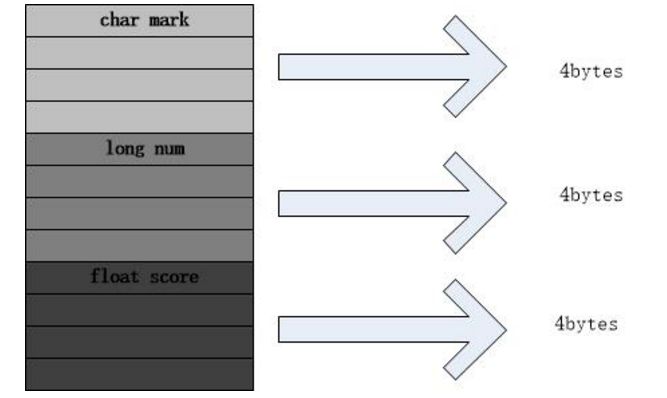
\includegraphics[width = 12cm]{struct.png}
				\caption{Struct 结构图}
			\end{figure} 
			
			sizeof(struct student)的值为12bytes.
		
		\subsection{函数使用}
			\subsubsection{传值}
		         \subparagraph{1. 使用引用改变}void Move(struct \& Parameter)
		         \subparagraph{2. 使用指针改变}void Move(struct * Parameter)
		         
		    \subsubsection{初始化}
			\begin{lstlisting}
	struct ListNode{
		int val;
		ListNode* next;		// 不用加struct 关键字
		ListNode(int i):val(i),next(nullptr){}	// 可以与类一样的定义构造函数
	};
	
	ListNode * ptr = new ListNode(0);	//不用typedef 就可以当类型用,如同类,可以理解为公开的类			
			\end{lstlisting} 
         
	\section{Union}     
        \subsection{定义} 
	        union又名共用体,假设定义结构为
	        \begin{lstlisting}
	union test
	{
		char mark;
		long num;
		float score;
	};
	
	union DATE
	{
		char a;
		int i[5];
		double b;
	};        
	        \end{lstlisting}
	        
	        则其结构如下:
	        \begin{figure}[h]
	        	\centering
	        	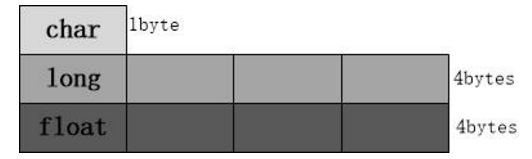
\includegraphics[width = 12cm]{union.png}
	        	\caption{Union test 结构图}
	        \end{figure} 
	        
	        sizeof(union test)的值为4bytes.原因如下:有的时候,我们需要几种不同类型的变量存在在同一段的内存空间中,就像上面的,我们需要将一个char类型的mark、一个long类型的num变量和一个float类型的score变量\textbf{存放在同一个地址开始的内存单元中}。
	        
	        上面的三个变量,char类型和long类型所占的内存字节数是不一样的,但是在union中,\textit{它们都是从同一个地址存放的,也就是使用的覆盖技术,这三个变量互相覆盖,而这种使几个不同的变量共占同一段内存的结构},称为“共用体”类型的结构
	        
	        结构体struct所占用的内存为各个成员的占用的内存之和(当然也需要考虑内存对齐的问题了)。而对于union来说,在谭浩强的《C语言程序设计》中这么说:\textbf{union变量所占用的内存长度等于最长的成员的内存长度}。
	        
	        它的\textbf{所有成员相对于基地址的偏移量都为0}。
	        
	        \begin{figure}[h]
	        	\centering
	        	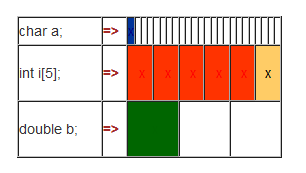
\includegraphics[width = 12cm]{union2.png}
	        	\caption{Union Date 结构图}
	        \end{figure}
	        
	        该结构要放得下int i[5]必须要至少占4×5=20个字节。如果没有double的话20个字节够用了,此时按4字节对齐。但是加入了double就必须考虑double的对齐方式,double是按照8字节对齐的,所以必须添加4个字节使其满足8×3=24,也就是必须也是8的倍数,这样一来就出来了24这个数字。综上所述,最终联合体的最小的size也要是所包含的所有类型的基本长度的最小公倍数才行。(这里的字节数均指win 下的值,平台、编译器不同值也有可能不同。)
	\section{字节对齐-StructAndUnion}
		不同编译器环境默认字节对齐的差别,做平台移植的同仁要注意了,遇到不确定的字节对齐问题,最好先亲自试一下,不能太想当然了:
		\begin{enumerate}
			\item Win32下,VC编译器默认8字节对齐,而且支持1、2、4、8、16五种对齐方式
			\item Linux 32下,GCC 4.1默认4字节对齐,支持1、2、4三种对齐方式。因此结构体中即使遇到double、long long这样的8字节变量,仍然按4字节对齐。即使设定了\#pragma pack(8),但在win32 下是8字节
		\end{enumerate}	        
         
\chapter{string} 
	\section{方法}
		\subsection{string类的构造函数}
			\begin{lstlisting}
	#include <iostream>
	#include <cassert>
	#include <iterator>
	#include <string>
	
	int main()
	{
		// 默认缺省构造
		{
			// string::string()
			std::string s;
			assert(s.empty() && (s.length() == 0) && (s.size() == 0));
		}
		
		// n 个相同字符
		{
			// string::string(size_type count, charT ch)
			std::string s(4, '=');
			std::cout << s << '\n'; // "===="
		}
		
		{
			std::string const other("Exemplary");
			// string::string(string const& other, size_type pos, size_type count)
			std::string s(other, 0, other.length()-1);
			std::cout << s << '\n'; // "Exemplar"
		}
		
		{
			// string::string(charT const* s, size_type count)
			std::string s("C-style string", 7);
			std::cout << s << '\n'; // "C-style"
		}
		
		{
			// string::string(charT const* s)
			std::string s("C-style\0string");
			std::cout << s << '\n'; // "C-style"
		}
		
		{
			char mutable_c_str[] = "another C-style string";
			// string::string(InputIt first, InputIt last)
			// 左闭右开
			std::string s(std::begin(mutable_c_str)+8, std::end(mutable_c_str)-1);
			std::cout << s << '\n'; // "C-style string"
		}
		
		{
			std::string const other("Exemplar");
			std::string s(other);
			std::cout << s << '\n'; // "Exemplar"
		}
		
		{
			// string::string(string&& str)
			std::string s(std::string("C++ by ") + std::string("example"));
			std::cout << s << '\n'; // "C++ by example"
		}
		
		{
			// string(std::initializer_list<charT> ilist)
			std::string s({ 'C', '-', 's', 't', 'y', 'l', 'e' });
			std::cout << s << '\n'; // "C-style"
		}
	}			
			\end{lstlisting}
		\subsection{string类的字符操作}
			\begin{itemize}
				\item \verb|operator[n]和at(n)|均返回当前字符串中第n个字符的位置,\textbf{但at函数提供范围检查},当越界时会抛出\verb|out_of_range|异常,下标\textbf{运算符[]不提供检查访问}
				\item \verb|bool empty() const;|Checks if the string has no characters, i.e. whether begin() == end()
				\item \verb|const char *data()const|;//返回一个非null终止的\textbf{不可修改的c字符数组}
				\item \verb|const char *c_str()const|;//返回一个以null终止的\textbf{不可修改的c字符串}
				\item \verb|int copy(char *s, int n, int pos = 0) const|;//把当前串中以pos开始的n个字符拷贝到以s为起始位置的字符数组中,返回实际拷贝的数目
				\item \verb|void push_back( CharT ch );|Appends the given character ch to the end of the string
				\item \verb|void pop_back();|Removes the last character from the string.
				\item \verb|stoi(), stof()| 将字符串转换为整数和浮点数
				\item \verb|std::to_string(num_type)| 将数字转换为字符串
			\end{itemize}
    \section{操作符}
         \subsection{+= 操作符}
	          \textbf{左边}只能是\verb|string字符串|,右边可以是string字符串,C风格的字符串、或是一个字符
         
         \subsection{+ 操作符}
	          \verb|+| 操作符的右边的两个不能都是字符串,\textbf{至少存在一个字符串对象}
         
	          \verb|s1 = "W.C." + "Fields";|                            //ERROR
         
         \subsection{== 操作符}
	         \verb|bool operator==(const string \&s1,const string \&s2)const|;//比较两个字符串是否相等
         
	         运算符">","<",">=","<=","!="均被重载用于字符串的比较;
         
    \section{宽字符 wchar\_t}
	    \begin{enumerate}
	    	\item  \verb|#include  1.stdlib.h  2.locale|
	    	\item  \verb|setlocale(LC_ALL,"chs");|
	    	\item  \verb|wchar_t *p = L"中文";|
	    \end{enumerate}
       
\chapter{class}
       
\section{C++ 中使用Struct 创建1个类}\verb|struct|关键字创建的类,类成员默认是公有的,但可以有私有的
	
	 new一个对象时, 只为类中成员变量分配空间, 对象之间共享成员函数。
	       
\section{C++ 中使用Class 创建1个类}\verb|class|关键字创建的类,类成员默认是私有的
	       
\section{const 型成员函数}\verb|int getAge()  const;|
	       \begin{enumerate}[fullwidth,itemindent=2em,label=(\arabic*)]
		       \item  会隐含第一个参数为this,即如果没有参数,实际类型为带有本身类型的一个参数。
		       \item  用于限制该函数,不允许该函数对任何数据成员进行修改。
		       
		       \item  一个\verb|const|成员函数仅能调用其他\verb|const|成员函数,因为\verb|const|成员不允许直接或间接的改变对象的状态,而调用非\verb|const|成员函数可能会间接的改变对象的状态
		       
		       \item 默认参数应在函数声明而非函数定义中给出:全部函数
	       \end{enumerate}
\section{析构函数与构造函数}
		\subsection{潜规则}
		    \begin{enumerate}[fullwidth,itemindent=2em,label=(\arabic*)]
		       \item  构造函数和析构函数比较特殊:在调用它们时不需要显式地提供函数名,编译器会自动调用它们
		       
		       \item  构造函数不能有返回值
		       
		       \item  构造函数主要用来对数据成员进行初始化,并负责其他一些在对象创建时需要处理的事务
		       
		       \item  自己定义构造函数,否则编译器会生成一个公有的构造函数
		    \end{enumerate}
		  \subsection{Initializer-List Constructors}    
			  \begin{lstlisting}
	class EvenSequence
	{
	public:
		EvenSequence(initializer_list<double> args)
		{
			if (args.size() % 2 != 0) {
			throw invalid_argument("initializer_list should "
				"contain even number of elements.");
			}
			mSequence.reserve(args.size());
				for (auto value : args) {
					mSequence.push_back(value);
				}
		}
		void dump() const
		{
			for (auto value : mSequence) {
				cout << value << ", ";
			}
			cout << endl;
		}	
	private:
		vector<double> mSequence;
	};
	
	EvenSequence p1 = {1.0, 2.0, 3.0, 4.0, 5.0, 6.0};
	p1.dump();
	try {
		EvenSequence p2 = {1.0, 2.0, 3.0};
	} catch (const invalid_argument& e) {
		cout << e.what() << endl;
	}
			  \end{lstlisting} 
	
	\subsection{初始化顺序}
		\begin{enumerate}
			\item 普通的变量:一般不考虑啥效率的情况下 可以在构造函数中进行赋值。考虑一下效率的可以再构造函数的初始化列表中进行
			\item static 静态变量
			\item const  常量变量:onst常量需要在声明的时候即初始化。一般采用在构造函数的初始化列表中进行。
			\item Reference 引用型变量:引用型变量和const变量类似。需要在创建的时候即进行初始化。也是在初始化列表中进行。但需要注意用Reference类型。
			\item 字符串初始化
		\end{enumerate}
\section{值语义与对象语义}
	\url{http://blog.csdn.net/chdhust/article/details/9927083}
	
	\subsection{值语义}
		所谓值语义是一个对象被系统标准的复制方式复制后,与被复制的对象之间毫无关系,可以彼此独立改变互不影响
	
	\subsection{对象语义}
		也叫指针语义,引用语义等,通常是指一个对象被系统标准的复制方式复制后,与被复制的对象之间依然共享底层资源,对任何一个的改变都将改变另一个
	
\section{拷贝构造函数} 拷贝构造函数创建一个新的对象,此对象是另外一个对象的拷贝品
	       \begin{enumerate}[fullwidth,itemindent=2em,label=(\arabic*)]		       
		       \item  \verb|Person(Person &)| ; 或 \verb|Person(const Person & )|;
		       
		       \item  如果类的设计者不提供拷贝构造函数,编译器会自动生成一个:\textit{将源对象所有数据成员的值逐一赋值给目标对象相应的数据成员}
		       
		       \item   通常,如果一个类包含指向动态存储空间指针类型的数据成员,则就应该为这个类设计拷贝构造函数(如果某个类定义了拷贝构造函数,类的设计者通常再为它添加一个赋值操作符重载函数)
		       
		       \item   浅拷贝即编译器提供的,只会拷贝值,\textbf{如果是数组的话,则是该数组的引用},而不重新分配空间。  
		 \end{enumerate}   
		       \subparagraph{浅拷贝与深拷贝}:
		       
		       1- 浅拷贝:两个对象之间成员变量简单的赋值。
		       
		       \begin{figure}[h]
		       	   \centering
		       	   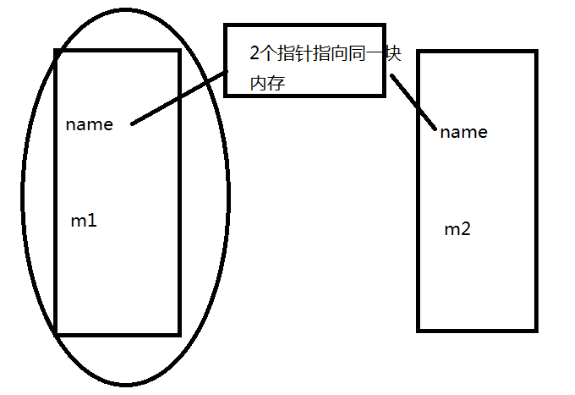
\includegraphics[width=8cm,clip]{weakCopy.png}
		       \end{figure}
		       
		       2- 深拷贝:不同的对象指针成员指向不同的内存地址,拷贝构造的时候不是简单的指针赋值,而是将内存拷贝过来。
		       
		       \subparagraph{拷贝构造函数可能的错误}
				     带实习的时候发现,一个同学写了一个类,没有写拷贝构造函数,然后在定义函数传参数时,用到该类型本身,结果就导致析构错误。 1种错误可能是因为该类型本身用了数组(默认拷贝构造函数数组是传引用的),导致释放重释放错误..非法操作地址
				     
				     2可能是 函数中(碰到\verb|return|;)的临时变量需要调用析构函数,而参数到函数结束时也会调用析构函数。
		       
\section{初始化列表}
	       
		       初始化列表仅在构造函数中有效,不能用于其他函数。构造函数的初始化列表可以初始化任何数据成员,但\verb|const|类型数据成员不能 用其他办法进行初始化
		       
		       数据成员初始化顺序完全取决于它们在类中声明的顺序(不是对应关系,是赋值的先后,对应还是一一对应),与它们在初始化段中出现的次序无关
		       
	       
\section{一些只有}
	       \begin{itemize}
		       \item 只能 \ 在成员函数 \ 或者\ friend函数中\textbf{访问类的 \ 非公有成员}
		       
		       \item 类成员或者非类成员  \   只有  \   静态变量被默认初始化
		       
		       \item \textbf{const成员}\ 必须在初始化段(列表)中被\textbf{初始化}
\begin{lstlisting}
	class Test{
	public:
		// ok: 必须这样
		Test() :testConst(1){}
		
		// error
		// Test() { testConst = 1; }
		
		// error
		// Test(){}
		const int testConst;
	};
	
	// error
	// int Test::testConst = 1;
	
	int main()
	{
		Test test;
		cout << test.testConst << endl;
		return 0;
	}
\end{lstlisting}

		       \item 指针this是一个常量,因此this作为赋值、递增、递减、操作符的目的对象都是错误的
		    \end{itemize}
	       
\section{STATIC 修饰词}
	\subsection{初始化时间}
		\textbf{全局}变量、\textbf{文件域}的静态变量和\textbf{类的静态成员}变量\textbf{在main执行之前}的静态初始化过程中分配内存并初始化;\textbf{局部静态变量}(一般为函数内的静态变量)\textbf{在第一次使用时分配内存并初始化}。这里的变量包含内置数据类型和自定义类型的对象。  
		
		 
		 \textbf{非局部静态变量}一般\textbf{在main执行之前}的静态初始化过程中分配内存并初始化,\textbf{可以认为是线程安全的}; 
	\subsection{静态全局变量}	
		       \begin{enumerate}[fullwidth,itemindent=2em,label=(\arabic*)]
			       \item  该变量在全局数据区分配内存
		       
			       \item  未经初始化的静态全局变量会被程序\textbf{自动初始化为0}(自动变量的值是随机的,除非它被显式初始化)
		       
			       \item  静态全局变量在声明它的整个文件都是可见的,而在文件之外是不可见的
		       
			       \item  全局数据区的数据并不会因为函数的退出而释放空间
		       \end{enumerate}
			       \textbf{->程序的内存分布}
		       
			       \quad  \color{red} {1- 代码区}
		       
			       \quad  \color{violet} {2- 全局数据区:静态数据(即使是函数内部的静态局部变量)也存放在全局数据区}
		       
			       \quad  \color{blue}{3- 堆区:由new产生的动态数据存放在堆区}
		       
			       \quad  \color{orange} {4- 栈区:函数内部的自动变量存放在栈区, 自动变量一般会随着函数的退出而释放空间}
			       \color{black}
	\subsection{静态局部变量}
		       \begin{enumerate}[fullwidth,itemindent=2em,label=(\arabic*)]
			       \item  在函数体内定义了一个变量,每当程序运行到该语句时都会给该局部变量分配栈内存。但随着程序退出函数体,系统就会收回栈内存,局部变量也相应失效。但有时候我们需要在两次调用之间对变量的值进行保存。通常的想法是定义一个全局变量来实现。但这样一来,变量已经不再属于函数本身了,不再仅受函数的控制,给程序的维护带来不便。
		       
			       \item  该变量在全局数据区分配内存
		       
			       \item  静态局部变量在程序执行到该对象的声明处时被首次初始化,即以后的函数调用不再进行初始化
		       
			       \item  静态局部变量一般在声明处初始化,如果没有显式初始化,会被程序自动初始化为0
		       
			       \item  它始终驻留在全局数据区,直到程序运行结束。但其作用域为局部作用域,当定义它的函数或语句块结束时,其作用域随之结束
		       \end{enumerate}
	\subsection{静态函数}
		       \begin{enumerate}[fullwidth,itemindent=2em,label=(\arabic*)]
			       \item  在函数的返回类型前加上\verb|static|关键字,函数即被定义为静态函数。静态函数与普通函数不同,它只能在声明它的文件当中可见,不能被其它文件使用
		       
			       \item  静态函数不能被其它文件所用
		       
			       \item  其它文件中可以定义相同名字的函数,不会发生冲突
		       \end{enumerate}
	\subsection{静态数据成员}
		       \begin{enumerate}[fullwidth,itemindent=2em,label=(\arabic*)]
			       \item  在类内数据成员的声明前加上关键字\verb|static|,该数据成员就是类内的静态数据成员
			       
			       \item  对于非静态数据成员,每个类对象都有自己的拷贝。而静态数据成员被当作是类的成员。无论这个类的对象被定义了多少个,静态数据成员在程序中也只有一份拷贝,由该类型的所有对象共享访问
			       
			       \item  静态数据成员存储在全局数据区。静态数据成员定义时要分配空间,所以不能在类声明中定义或初始化,同其他一样在\verb|cpp|文件中初始化
			       
			       \item  静态数据成员和普通数据成员一样遵从\verb|public,protected,private|访问规则
		       \end{enumerate}
		       
	\subsection{静态成员函数}
		       \begin{enumerate}[fullwidth,itemindent=2em,label=(\arabic*)]
			       \item  静态成员函数与静态数据成员一样,都是类的内部实现,属于类定义的一部分。普通的成员函数一般都隐含了一个\verb|this|指针,\verb|this|指针指向类的对象本身,因为普通成员函数总是具体的属于某个类的具体对象的,但是与普通函数相比,静态成员函数由于不是与任何的对象相联系,因此它不具有\verb|this|指针,从这个意义上讲,它\textbf{无法访问}属于类对象的\textit{非静态数据成员},也无法访问\textit{非静态成员函数},它\textbf{只能调用}其余的\textit{静态成员函数}。
			       
			       \item  出现在类体外的函数定义不能指定关键字\verb|static|,即声明函数时加\verb|static| ,在外面实现时不加
			       
			       \item  由于没有\verb|this|指针的额外开销,因此静态成员函数与类的全局函数相比速度上会有少许的增长
		       \end{enumerate}

\chapter{this}
	\section{概念}
	
	\section{易混问题}
		\url{https://www.cnblogs.com/lijia0511/p/4936843.html}
		       
\chapter{继承}
\section{潜规则}
	       \begin{enumerate}[fullwidth,itemindent=2em,label=(\arabic*)]
	       	\item   不指明继承方式关键字\verb|public|时,编译器会默认继承方式为\verb|private|或\verb|protected|
	       	\item   基类的所有私有成员仅在基类中可见,而在派生类中是不可见的。基类的私有成员可以由派生类继承,但是派生类不可见
	       	\item   继承相当于把父类所有的东西复制了一份,但是可能因访问权限的设置而不能使用。
	       	\item   公有继承的保护成员,\textbf{只能在派生类中访问,不能用派生类对象访问}
	       	\item   如果派生类添加了一个数据成员,而该成员与基类中的某个数据成员同名,新的数据类型就  隐藏  了继承来的同名成员;同理,函数也存在隐藏
	       	\item   派生类可对从基类继承来的保护成员进行访问,也就是说保护成员在派生类中是可见的 ,但是只能在对象内部进行调用,但是不能通过对象在外部调用
	       	
	       	例子:
		       	 \begin{lstlisting}[language={[ANSI]C++}]
	class BC
	{
	public:
		void set_x(int a){x=a;}
	
	protected:
		int get_x() const {return x;}
	private:
		int x;
	};
	
	class DC:public BC
	{
	public:
		void add2() {int c = get_x(); set_x(c+2);}  //Right Can read protected variable
	};
	
	int main()
	{
		DC d;
		d.set_x(3);
		//cout << d.get_x() << endl;     //Wrong! can not run,use the protected method out Object
		// d.x = 77;                     //Wrong! can not run
		d.add2();
		
		return 0;
	}	       	
		       	\end{lstlisting}
	       \qquad \color{blue}	{main函数中能够访问DC的公有成员set\_x和add2,但不能访问保护成员get\_x,get\_x仅在类层次结构中可见 (不能以对象的方式访问)}
	       
	       \color{black}  \item  {除了friend函数,只有处于类层次结构中的成员函数才能访问保护成员[派生]}
	     
	       \item 应避免将数据成员设计为保护类型,即使某个数据成员可 以成为保护成员,但更好的解决方案是:首先将这个数据成员定义为私有成员,然后为它设计一个用来进行存取访问的保护成员函数
	      
	       \item 可以使用 基类指针 存贮 子类.但是 不能调用子类相关的 函数:
		       \begin{lstlisting}
	class Super
	{
	public:
		Super();
		void someMethod();
	protected:
		int mProtectedInt;
	private:
		int mPrivateInt;
	};
	
	class Sub : public Super
	{
	public:
		Sub();
		void someOtherMethod();
	};
	
	Super mySuper;
	mySuper.someOtherMethod(); // Error! Super doesn't have a someOtherMethod().
	
	Super* superPointer = new Sub(); // Create sub, store it in super pointer.
	superPointer->someOtherMethod(); // Error! However, you CanNot call methods from the Sub class through the Super pointer. 
		       \end{lstlisting}
	       \end{enumerate}
     
\section{构造函数调用顺序}
	       \begin{enumerate}[fullwidth,itemindent=2em,label=(\arabic*)]
	       	 \item 当创建一个派生类时,基类的构造函数被自动调用,用来对派生类对象中的基类部分初始化,并完成其他一些相关事务,但是必须在派生类的构造函数处明确优先调用\textbf{,:super(),you}
	       	 \item 在类的层次结构中,构造函数按基类到派生类的次序执行,析构函数则按派生类到基类的次序执行
	       \end{enumerate}
 
\section{继承方式}
	\subsection{继承后对父类资源的访问权限}
		各种继承后,派生类\textbf{对父类资源的访问权限}变为如图所示:
		\begin{figure}[h]
			\centering 
			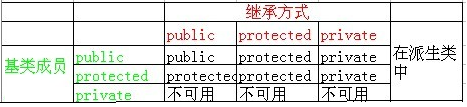
\includegraphics[scale = 0.8]{derive.png}
		\end{figure}   
		   
	\subsection{继承约束}
		\subsubsection{禁止继承-final}
			将类定义为 \verb|final | 意味着该类将不再允许被继承.
			\begin{lstlisting}
	class Super final
	{
		// Omitted for brevity
	};
	
	// The following Sub class tries to inherit from the Super class, but this will result in a compiler error because Super is marked as final.
	class Sub : public Super
	{
		// Omitted for brevity
	};
			\end{lstlisting}
			
	\subsection{重写 父类方法}
			\textbf{Only} methods that \textbf{are declared as} \verb|virtual| in the base class \textbf{can be} overridden properly by derived classes.
			
			If you wish to \textbf{provide a new definition} for \verb|someMethod()| in the \verb|Sub class|, you must first \textbf{add it} \textit{to} the class \textbf{definition} for \verb|Sub|,as follows:
		
			\begin{lstlisting}
	class Sub : public Super
	{
	public:
		Sub();
		virtual void someMethod() override; // Overrides Super's someMethod()
		virtual void someOtherMethod();
	};
	
	void Sub::someMethod()
	{
		cout << "This is Sub's version of someMethod()." << endl;
	}
			\end{lstlisting}
		
		\textbf{Once} \verb|a method| or \verb|destructor| is \textbf{marked} as \verb|virtual|, it will be \verb|virtual| for all derived classes even if the \verb|virtual| keyword is removed from derived classes
		
			\begin{lstlisting}
	class Sub : public Super
	{
	public:
		Sub();
		void someMethod() override; // Overrides Super's someMethod()
	};
			\end{lstlisting}
			
	\subsection{切片} 
			当用 \textbf{基类指针 或 引用} 子类对象,此时\textbf{可以调用} \textit{基类存在的函数或成员},但是\textbf{不能调用}子类 \textbf{独有的}函数与数据成员, 但当调用 \textbf{赋值操作符} 进行构造对象,那么此时对象调用的函数 \textbf{将是基类原版本},而非子类重写的版本
			
			\begin{lstlisting}
	Super mySuper;
	mySuper.someMethod(); // Calls Super's version of someMethod().
	
	Sub mySub;
	mySub.someMethod(); // Calls Sub's version of someMethod()
	
	Sub mySub;
	Super& ref = mySub;
	ref.someMethod(); // Calls Sub's version of someMethod()
	
	Sub mySub;
	Super& ref = mySub;
	mySub.someOtherMethod(); // This is fine.
	ref.someOtherMethod(); // Error
	
	Sub mySub;
	Super assignedObject = mySub; // Assigns a Sub to a Super.
	assignedObject.someMethod(); // Calls Super's version of someMethod()
			\end{lstlisting}
			
			\begin{lstlisting}[frame = lTbr]
    Derived classes retain their overridden methods when referred to by base class pointers or references. They lose their uniqueness when cast to a base class object. The loss of overridden methods and derived class data is called slicing.
			\end{lstlisting}
			
			\subparagraph{Casting Up and Down}
				When upcasting, \textbf{use a pointer or reference} to the base class \textbf{to avoid slicing}.
				
			\begin{lstlisting}
	Super mySuper = mySub; // SLICE!
	Super& mySuper = mySub; // No slice!
	
	void lessPresumptuous(Super* inSuper)
	{
		// Use downcasting only when necessary and be sure to use a dynamic_cast.
		Sub* mySub = dynamic_cast<Sub*>(inSuper); 	
		if (mySub != nullptr) {
			// Proceed to access Sub methods on mySub.
		}
	}
			\end{lstlisting}
			
	\subsection{使用 父类方法}	
		\begin{lstlisting}
	class B: public A {
	public:
	void func3(string prefix) {
			cout << prefix << "B::func3" << endl;
			A::func3(prefix + "  ");
		}
	};
		\end{lstlisting}
				
\section{支持多继承}一个派生类可以拥有多个基类
	        \begin{enumerate}[fullwidth,itemindent=2em,label=(\arabic*)]
	          \item 多继承中,多个基类每个基类都要加上访问修饰符,缺省则默认为私有的
	        \end{enumerate}
        
\section{虚基类}使用虚基类能够在多重派生的过程中,\textbf{使共有的基类部分在派生类中只有一个拷贝},这样就能解决二义性的错误。
		        \begin{figure}[h]
		        	\begin{center}
		        		\begin{minipage}[H]{0.5\textwidth}
			        			\centering
			        			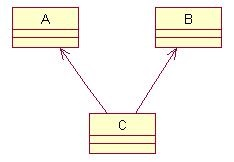
\includegraphics[angle=0,width=8cm,height=5.6cm]{derive.jpg}%就在前面括号中写图片名
			        			\caption{普通多继承}
			        			\label{fig:derive}
		        		\end{minipage}%
		        		\begin{minipage}[H]{0.5\textwidth} 
			        			\centering
			        			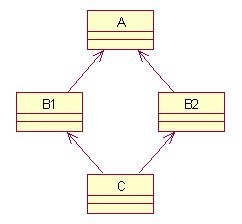
\includegraphics[angle=0,width=8cm,height=5.6cm]{derive2.jpg}
			        			\caption{二义性多继承}
			        			\label{fig:derive2}
		        		\end{minipage}
		        	\end{center}
		        \end{figure}
        
		        \begin{lstlisting}
	class A
	{
	public:
		A(int a = 0) : mA(a) {}
		int mA;
	};
	
	class B1 : virtual public A
	{
	public:
		B1(int a = 0, int b = 0) : A(b), mB1(a) {}
		int mB1;
	};
	
	class B2 : virtual public A
	{
	public:
		B2(int a = 0, int b = 0) : A(b), mB2(a) {}
		int mB2;
	};
	
	class C : public B1, public B2
	{
	public:
		C(int x, int a, int b, int c, int d) : B1(a, b), B2(c, d), mC(x) {}
		
		void Print() const
		{
			cout << "B1::mA = " << B1::mA << endl;
			cout << "B2::mA = " << B2::mA << endl;
			cout << "mA = " << mA << endl;
			cout << "mB1 = " << mB1 << endl;
			cout << "mB2 = " << mB2 << endl;
			cout << "mC = " << mC << endl;
		}
		
		int mC;
	};
	
	int main()
	{
		C obj(10, 20, 30, 40, 50);
		obj.Print();
		cout << endl;
		obj.mA = 163;
		obj.Print();
		return 0;
	}
	
	---------------Output------------- :
		B1::mA = 0
		B2::mA = 0
		mA  = 0
		mB1 = 20
		mB2 = 40
		mC  = 10
		
		B1::mA = 163
		B2::mA = 163
		mA  = 163
		mB1 = 20
		mB2 = 40
		mC  = 10	       	
		        \end{lstlisting} 
        
	        \begin{enumerate}[fullwidth,itemindent=2em,label=(\arabic*)]
	        	
		        \item 共有部分 为mA; 私有部分 为mBx; 共有部分调用基类进行初始化(没有显示调用基类)	
		        
		        \item 虚基类的构造函数的调用方法与一般基类的构造函数的调用方法是不同的。在这个例子中,编译器没有调用B1或者B2的构造函数来调用基类A的构造函数,因为在虚继承过程中,基类A只有一个拷贝,所以编译器无法确定应该由类B1或者类B2的构造函数来调用基类A的构造函数,所以此时调用的是基类A的默认构造函数,所以刚开始mA的结果为0,是基类A的默认构造函数设置的默认值。
		        
		        \item  由虚基类经过一次或者多次派生出来的派生类,在其每一个派生类的构造函数的成员初始化列表中必须给出对虚基类的构造函数的调用,如果未列出,则调用虚基类的默认构造函数。
		        
		        \item 在本例当中,在执行B1和B2的构造函数时都不调用虚基类A的构造函数,而是在类C中的构造函数直接调用虚基类A的默认构造函数。
		        
		        \item \textbf{如果将C的构造函数改为C(int x, int a, int b, int c, int d) : A(a), B1(a, b), B2(c, d), mC(x) {},则在这里显示地调用虚基类A的构造函数},并传入初始值,所以第一次打印mA的值不是0,而是20。
		        
	        \begin{lstlisting}
	------------------Output---------------
		B1::mA = 20
		B2::mA = 20
		mA  = 20
		mB1 = 20
		mB2 = 40
		mC  = 10
		
		B1::mA = 163
		B2::mA = 163
		mA  = 163
		mB1 = 20
		mB2 = 40
		mC  = 10        
	        \end{lstlisting}
	         
	      \end{enumerate}
        
\section{C++接口的实现方式}
	接口即\textbf{只包含}\textit{纯虚函数}的抽象类
	
	\subsection{纯虚函数}
		纯虚函数是在基类中声明的虚函数,它在基类中没有定义,但要求任何派生类都要定义自己的实现方法。在基类中实现纯虚函数的方法是在函数原型后加\verb|“=0”|
		$$\verb| virtual 返回值类型成员函数名(参数表)=0;|$$
		
	\subsection{抽象类}
		\textbf{包含}\verb|纯虚函数|的类称为抽象类。由于抽象类\textbf{包含了}没有定义的纯虚函数,所以\textbf{不能定义抽象类的对象}
      
	    重要的是抽象类\textbf{可以包括}抽象方法,这是\textbf{普通类所不能的},\textit{但同时也能}\textbf{包括普通的方法}。
	    
	    抽象方法只能声明于抽象类中,且不包含任何实现,\textbf{派生类必须覆盖它们}
	    
	 \subsection{C++ 接口与抽象类的区别}
		 \url{http://blog.csdn.net/hackbuteer1/article/details/7558946}
		 
		 
\chapter{virtual  关键字}
\section{多态}实际上是一个函数指针,在运行期间把该函数指针指向子类的相同函数
		
		\subparagraph{编译器绑定-非多态}一个函数的名称和其入口地址是紧密相连的,入口地址是该函数在内存中的起始地址
		
		由于函数被调用时,到底应该执行哪一段代码是由编译器在编译阶段就决定了的,因此我们将这种对函数的绑定方式称为编译器绑定(compile-time  bindinig):专业术语:编译器将所以对函数的调用绑定到函数的入口地址
		
		\subparagraph{运行期绑定-多态}与编译器绑定不同的时,运行期绑定是直到程序运行之时,才将函数名称绑定到其入口地址。
		
		如果对一个函数的绑定发生在运行期而非编译器,我们就称该函数是   多态
		
		\subparagraph{C++中多态有以下三个前提条件}:
			\begin{enumerate}[fullwidth,itemindent = 2em]
				\item 必须存在一个继承体系结构
				\item 继承体系结构中的一些类型必须具有同名的 \verb|virtual| 成员函数(virtual关键字)
				\item 至少有一个基类类型的指针或基类类型的引用,这个指针或引用可用来对virtual成员函数进行调用
			\end{enumerate}
		
		\subparagraph{*析构函数为什么要是 virtual的}在公有继承中,基类对派生类及其对象的操作,只能影响到那些从基类继承下来的成员.如果想要用基类对非继承成员进行操作,则要把基类的这个函数定义为虚函数.
			
			析构函数自然也应该如此:如果它想析构子类中的重新定义或新的成员及对象,当然也应该声明为虚的.
			
		\subparagraph{占用空间问题}C++中虚函数的实现使用到了虚表,如果一个类的成员函数有虚函数,因为要存储虚表指针,其占用的空间会比存储所有数据成员所需要的内存空间大,从而造成与C语言中的结构体内存占用不一样,最终与C语言不兼容。
		
		为了兼容C语言,C++实现的方式是对于所有无虚函数的类,都没有虚表指针,从而这样的类与C语言的结构体是可以兼容的。
		
		一般是一个int 的字节(4); 
		
		\textbf{深入c++ 内存模型}:\url{http://blog.csdn.net/qingyuanluofeng/article/details/48015901}

\section{虚函数表}
		\url{http://www.cnblogs.com/hushpa/p/5707475.html#undefined}
		
		\subparagraph{vtbl}
		每一个class 产生出一堆 指向\verb|virtual functions| 的指针,放在表格之中。这个表格被称为 \verb|virtual table(vtbl)|.
		\subparagraph{vptr}
		每个\verb|class object| 被安插一个指针,指向相关的\verb|virtual table|. 通常这个指针被称为 \verb|vptr|. \verb|vptr| 的设置 和 重置 都由每一个 class 的 constructor、deconstructor 和 copy assignment 运算符自动完成. 每个class 所关联的 \verb|type_info object|(用以 支持\verb|runtime type identification, RTTI|) 也经由 \verb|virtual table| 被指出来,通常该指针放在表格的 第一个\verb|slot|.
					
		虚函数(\verb|Virtual Function|)是通过一张虚函数表(\verb|Virtual Table|)来实现的。简称为\verb|V-Table|。在这个表中,主是要一个类的虚函数的地址表,这张表解决了继承、覆盖的问题,保证其容真实反应实际的函数。这样,在有虚函数的类的实例中这个表被分配在了这个实例的内存中,所以,当我们用父类的指针来操作一个子类的时候,这张虚函数表就显得由为重要了,它就像一个地图一样,指明了实际所应该调用的函数。	
		
		
        C++的编译器应该是保证虚函数表的指针存在于对象实例中最前面的位置,这意味着\textbf{我们通过对象实例的地址得到这张虚函数表,然后就可以遍历其中函数指针,并调用相应的函数}。
        
        
        \textbf{同属于一个类}的\textit{对象}\textbf{共享虚函数表}, 但是有各自的\verb|_vptr|
        \begin{lstlisting}
	class Base {
	public:
		virtual void f() {cout<<"base::f"<<endl;}
		virtual void g() {cout<<"base::g"<<endl;}
		virtual void h() {cout<<"base::h"<<endl;}
	};
	
	class Derive : public Base{
	public:
		void g() {cout<<"derive::g"<<endl;}
	};
	
	//可以稍后再看
	int main () {
		cout<<"size of Base: "<<sizeof(Base)<<endl;
		
		typedef void(*Func)(void);
		Base b;
		Base *d = new Derive();
		
		long* pvptr = (long*)d;
		long* vptr = (long*)*pvptr;
		Func f = (Func)vptr[0];
		Func g = (Func)vptr[1];
		Func h = (Func)vptr[2];
		
		f();
		g();
		h();
		
		return 0;
	}
	
	
	/*   Output  */
	size of Base: 8
	base::f
	derive::g
	base::h
        \end{lstlisting}
        
       \textbf{new一个对象时}, 只为类中成员变量分配空间, 对象之间共享成员函数。
        
       运行下上面的代码发现\verb|sizeof(Base) == 8|, 说明编译器在类中自动添加了一个8字节的成员变量, 这个变量就是\verb|_vptr|, 指向虚函数表的指针。
       
       \begin{enumerate}
	       	\item \verb|d|对象的首地址就是\verb|vptr|指针的地址-\verb|pvptr|
	       	\item 取\verb|pvptr|的值就是\verb|vptr|-虚函数表的地址
	       	\item 取\verb|pvptr|的值 等价于 \verb|*d|
	       	\item 取\verb|vptr中[0][1][2]|的值就是这三个函数的地址,通过函数地址就直接可以运行三个虚函数了。
	       	\item 函数表中\verb|Base::g()|函数指针被\verb|Derive|中的\verb|Derive::g()|函数指针覆盖, 所以执行的时候是调用的\verb|Derive::g()|
       \end{enumerate}
       
       \begin{figure}[h]
       	\centering
       	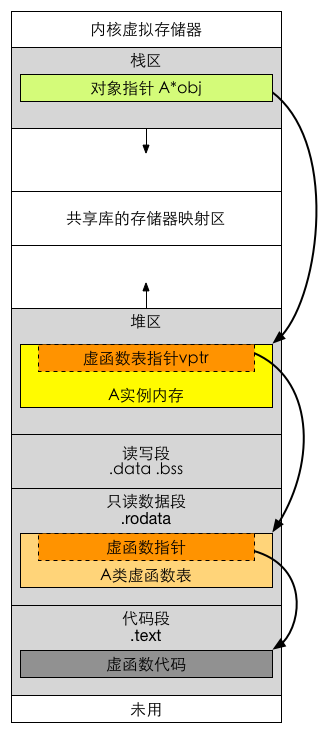
\includegraphics[scale=0.8]{process.png}
       	\caption{进程虚拟内存图-对象结构}
       \end{figure}
       
      \subsection{一般继承(无虚函数覆盖)}
	      对于实例:\verb|Derive d;| 的虚函数表如图\ref{vir-no}:
	      
		      \begin{figure}[h]
		      	\centering
		      	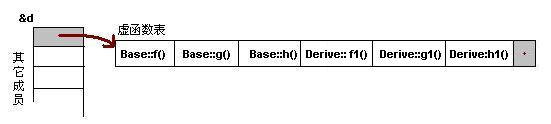
\includegraphics[scale=0.8]{vt-base.jpg}
		      	\caption{一般继承(无虚函数覆盖)\label{vir-no}}
		      \end{figure}
		     
		     \begin{itemize}
		     	\item 虚函数按照其声明顺序放于表中
		     	\item 父类的虚函数在子类的虚函数前面
		     \end{itemize}
      \subsection{一般继承(有虚函数覆盖)}
        为了看到被继承过后的效果,在这个类的设计中,我只覆盖了父类的一个函数:\verb|f()|。那么,对于派生类的实例,其虚函数表会是下面图\ref{vir-yes}的一个样子:
        
	         \begin{figure}[h]
	         	\centering
	         	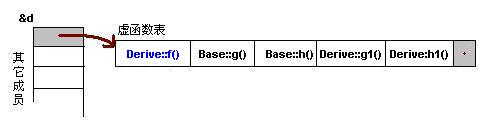
\includegraphics[scale=0.8]{vt-base2.jpg}
	         	\caption{一般继承(有虚函数覆盖)\label{vir-yes}}
	         \end{figure}
	         
	         \begin{itemize}
	         	\item 覆盖的f()函数被放到了虚表中原来父类虚函数的位置
	         	\item 没有被覆盖的函数依旧
	         \end{itemize}
	         
	         这样,我们就可以看到对于下面这样的程序\verb|  Base *b = new Derive();| \verb|b->f();|由\verb|b|所指的内存中的虚函数表的\verb|f()|的位置已经被\verb|Derive::f()|函数地址所取代,于是在实际调用发生时,是\verb|Derive::f()|被调用了。这就实现了\textbf{多态}。

	
\chapter{C++ 内存结构}
	\section{进程结构}
		\begin{figure}[htbp]
			\centering
			\includegraphics[scale=0.7]{processMem.png}
			\caption{进程内存结构}
		\end{figure}
		
		\subsection{Stack 栈}
			栈,存放\verb|Automatic Variables|,按内存地址由高到低方向生长,其最大大小由编译时确定,速度快,但自由性差,最大空间不大。
		
		\subsection{Heap 堆}
			堆,自由申请的空间,按内存地址由低到高方向生长,其大小由系统内存/虚拟内存上限决定,速度较慢,但自由性大,可用空间大。 
			
			\textbf{每个线程都会有自己的栈,但是堆空间是共用的。}
			
			堆和栈都是动态分配内存,两者空间大小都是可变的。
		\subsection{.bss 未初始化全局与静态变量}
			存放程序中未初始化的和零值全局变量与静态变量。静态分配,在程序开始时通常会被清零。
			
		\subsection{.data 初始化的全局与静态变量}
			用来存放程序中已经初始化的非零全局变量与静态变量。静态分配
			
			data又可分为读写(RW)区域和只读(RO)区域。 
			\begin{itemize}[itemindent = 2em]
				\item \verb|RO|段保存常量所以也被称为\verb|.constdata |
				\item \verb|RW|段则是普通非常全局变量,静态变量就在其中
			\end{itemize}
			
		\subsection{.text 代码区}
			也称为代码段(\verb|Code|),用来存放程序执行代码,同时也可能会包含一些常量(如一些字符串常量等)。该段内存为静态分配,只读(某些架构可能允许修改)。 
			
			这块内存是共享的,当有多个相同进程(\verb|Process|)存在时,共用同一个\verb|.text|段。
			
			\verb|text|和\verb|data|段都在可执行文件中,\textbf{由系统从可执行文件中加载};而\verb|bss|段不在可执行文件中,\textbf{由系统初始化。} 
			这三段内存就组成了我们编写的程序的本体
	\section{对象结构}
		\url{http://www.cnblogs.com/gtarcoder/p/4929927.html}
		
		\url{http://www.cnblogs.com/jerry19880126/p/3616999.html}
		
		\subsection{虚函数在内存中分布}
			对于有虚函数的基类和子类来说,内存中类对象的开始位置就是4字节的\verb|VPTR|(虚函数表的地址,指向\verb|VTABLE|)。
			
			\textit{如果一个子类继承自基类,且没有对虚函数进行重写},子类\textbf{仍然会自己维护一个虚函数表},和基类的虚函数表地址不同(尽管可能内容相同)。 
			
			\color{blue}可以这样理解,每个类都是一个架构模型,不同类型的实例则是需要根据不同的架构进行填充内存的。所以每个类都需要有各自的架构模型,如果是继承那么会将父类的模型拷贝过来再改造。
			\color{black}
			
			
			\textbf{虚函数表中存放该类对应的实际会调用的函数地址,} \textit{即若子类没有覆盖基类的虚函数,则对应位置存放基类虚函数地址};\color{blue}\textbf{若子类覆盖了基类的虚函数,则对应位置存放子类的虚函数地址}。虚函数表以\verb|NULL|结尾。且如果子类中添加了基类中没有的虚函数,则新加的虚函数被放在子类虚函数表最后。 \color{black}
			
			\textbf{虚函数表只存放虚函数的地址,非虚函数由编译器在编译期间静态设定。} 
			
			\textbf{如果一个子类是多继承},即含有多个基类,\textbf{则有多个虚函数表,分别对应到不同的继承}。

		
		\subsection{单一对象}
		
			\begin{lstlisting}
	class Base
	{
		int a;
		int b;
		public:
		void CommonFunction();
	};			
			\end{lstlisting}
			\begin{figure}[ht]
				\centering
				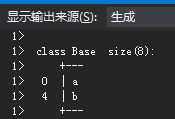
\includegraphics[scale = 0.8]{figure/single.png}
				\caption{单一对象}
			\end{figure}
			 c++类中有四种成员:
				\begin{enumerate}[itemindent = 1em]
					\item 非静态数据成员:放在每个对象内部,作为对象专有的数据成员
					\item 静态数据成员:被抽取出来放在程序的静态数据区内,\textbf{为该类所有对象共享,只保留一份} 
					\item 非静态成员函数:
					\item 静态成员函数:都被提取出来放在程序的代码段中并为该类\textbf{所有对象共享},因此每个成员函数也只能存在一份代码实体
				\end{enumerate}
			 
				   因此,构成对象的只有数据,任何成员函数都不属于任何一个对象,非静态成员函数和对象的关系就像是绑定,绑定的中介就是this指针。而this 指针是以默认的类指针 对象作为第一个参数传进成员函数的,所以不占空间。
				   
				   $$ \verb|对象大小 = 非静态数据成员|$$
		
		\newpage
	\subsection{单一对象(virtual)}
		\begin{lstlisting}
	class Base
	{
		int a;
		int b;
	public:
		void CommonFunction();
		void virtual VirtualFunction();
	};			
		\end{lstlisting}
	
	\begin{figure}[ht]
		\centering
		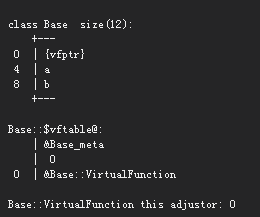
\includegraphics[scale = 0.8]{figure/singleVirtual.png}
		\caption{单对象,包含虚函数}
	\end{figure}

		
		\newpage			   
		\subsection{单继承(base 无virtual)}		   
			\begin{lstlisting}
	class DerivedClass: public Base
	{
		int c;
		public:
		void DerivedCommonFunction();
	};
			\end{lstlisting}
			
			\begin{figure}[ht]
				\centering
				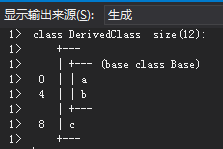
\includegraphics[scale = 0.8]{figure/singleDerived.png}
				\caption{单继承}
			\end{figure}
	
		\newpage
		\subsection{单继承(base 有virtual)}DerivedClass继承了Base,内存排布是\textbf{先父类后子类}。
		    \begin{lstlisting}
	class DerivedClass: public Base
	{
		int c;
		public:
		void DerivedCommonFunction();
		void virtual VirtualFunction();
	};	      	
		    \end{lstlisting}
		      
		    \begin{figure}[ht]
		      \centering
		      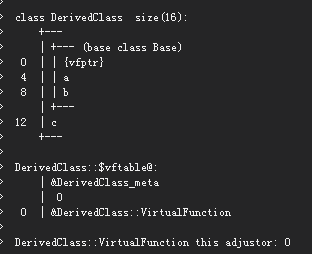
\includegraphics[scale = 0.8]{figure/singleDerivedVirutal.png}
		      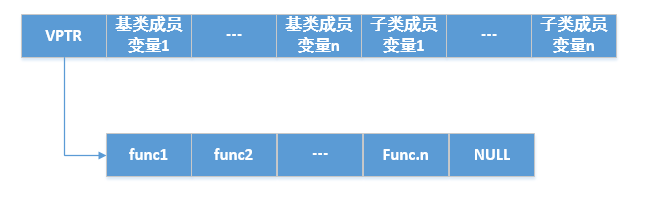
\includegraphics[scale = 0.8]{vtable1.png}
		      \caption{单继承,包含虚函数}
		    \end{figure}  	

		\newpage
		\subsection{虚继承-单继承(virtual)}
			\begin{lstlisting}
	class DerivedClass1: virtual public Base
	{
		int c;
	public:
		void DerivedCommonFunction();
		void virtual VirtualFunction();
	};
	
	class DerivedClass2 : virtual public Base
	{
		int d;
	public:
		void DerivedCommonFunction();
		void virtual VirtualFunction();
	};
	
	class DerivedDerivedClass :  public DerivedClass1, public DerivedClass2
	{
		int e;
	public:
		void DerivedDerivedCommonFunction();
		void virtual VirtualFunction();
	};
			\end{lstlisting}
		
		\begin{figure}[ht]
			\centering
			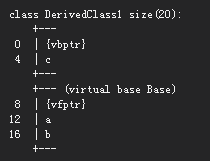
\includegraphics[scale = 0.8]{figure/virtualDerivedVirutal.png}
			\caption{虚单继承,包含虚函数}
		\end{figure}

	\newpage	
		\subsection{多继承(base  有 virtual)}
			如果一个子类有多个基类,为多继承。
			
			\textbf{其对象在内存中的布局为}:
				\begin{enumerate}
					\item \textit{按照多个继承,分为多个块};
					\item \textbf{每块的开头为一种继承的虚函数表},接着为该种继承的基类的非静态成员变量
					\item 所有块结束之后,为该子类特有的非静态成员变量
					\item 如果该子类又新加了虚函数,则虚函数\textbf{放在第一个虚函数表的最后}。
				\end{enumerate}
			
			\begin{lstlisting}
// 显示菱形继承
	class Base
	{
		int a;
		int b;
		public:
		void CommonFunction();
		void virtual VirtualFunction();
	};
	
	
	class DerivedClass1: public Base
	{
		int c;
		public:
		void DerivedCommonFunction();
		void virtual VirtualFunction();
	};
	
	class DerivedClass2 : public Base
	{
		int d;
		public:
		void DerivedCommonFunction();
		void virtual VirtualFunction();
	};
	class DerivedDerivedClass : public DerivedClass1, public DerivedClass2
	{
		int e;
		public:
		void DerivedDerivedCommonFunction();
		void virtual VirtualFunction();
	};	
	
	
// 验证子类新建虚函数位置 添加在 第一张虚表上
	class A{
		public:
		virtual void f1(){
			cout << "f1 in class A" << endl;
		}
		private:
		int a;
	};
	class B{
		public:
		virtual void f2(){
			cout << "f2 in class B" << endl;
		}
		virtual void f4(){
			cout << "f4 in class B" << endl;
		}
		int b;
	}
	class D:public A, B{
		public:
		void f1(){
			cout << "f1 in class D" << endl;
		}
		void f2(){
			cout << "f2 in class D" << endl;
		}
		virtual void f3(){
			cout << "f3 in class D" << endl;
		}
		private:
		double c;
	}		
			\end{lstlisting}
			
			\begin{figure}[ht]
				\centering
				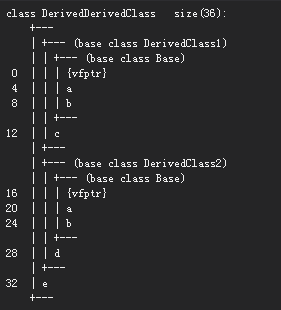
\includegraphics[scale = 0.8]{figure/DerivedDerivedVirutal.png}
				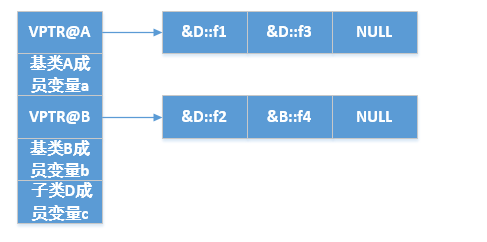
\includegraphics[scale = 0.8]{vtable2.png}
				\caption{多继承,包含虚函数}
			\end{figure}
			
			由外向内看,它并列地排布着继承而来的两个父类DerivedClass1与DerivedClass2,还有自身的成员变量e。DerivedClass1包含了它的成员变量c,以及Base,Base有一个0地址偏移的虚表指针,然后是成员变量a和b;DerivedClass2的内存排布类似于DerivedClass1,\textbf{注意到DerivedClass2里面竟然也有一份Base。}
			
			\subparagraph{菱形继承}如果有多个类继承自同一个基类,最后又被同一个子类继承这些类(例如 B, C继承自A, D继承自B,C),这种情况下,若类型A存在非静态成员变量a,则会有D类型的对象保留从B继承来的a和从C继承来的a,出现空间冗余。 
			
			\textbf{使用虚继承},可以使得D从B继承来的a和从C继承来的a是同一个,\textbf{节省空间}。 

		\newpage
		\subsection{虚继承-多继承(base  有 virtual)}
			\begin{lstlisting}
	class Base
	{
		int a;
		int b;
		public:
		void CommonFunction();
		void virtual VirtualFunction();
	};	
	
	class DerivedClass1: virtual public Base
	{
		int c;
		public:
		void DerivedCommonFunction();
		void virtual VirtualFunction();
	};
	
	class DerivedClass2 : virtual public Base
	{
		int d;
		public:
		void DerivedCommonFunction();
		void virtual VirtualFunction();
	};
	
	class DerivedDerivedClass :  public DerivedClass1, public DerivedClass2
	{
		int e;
		public:
		void DerivedDerivedCommonFunction();
		void virtual VirtualFunction();
	};
			\end{lstlisting}
			
			\subparagraph{Derived类图}
			
				\verb|DerivedClass1|就已经有变化了,原来是先排虚表指针与\verb|Base|成员变量,\verb|vfptr|位于0地址偏移处;但现在有两个虚表指针了,一个是\verb|vbptr|,另一个是\verb|vfptr|。\verb|vbptr|是这个\verb|DerivedClass1|对应的虚表指针,它指向\verb|DerivedClass1|的虚表\verb|vbtable|,另一个\verb|vfptr|是虚基类表对应的虚指针,它指向\verb|vftable|。
				
				\begin{figure}[ht]
					\centering
					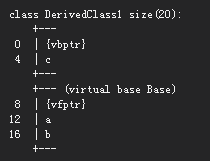
\includegraphics[scale = 0.8]{Derived.png}
					\caption{虚多继承-D}
				\end{figure}
			
			\subparagraph{DerivedDerived  类图}
				
				这里面有三个虚指针了,但\verb|base|却只有一份。第一张虚表是内含\verb|DerivedClass1|的,第二张虚表是内含\verb|DerivedClass2|的,最后一张表是虚基表。
				
				\begin{figure}[ht]
					\centering
					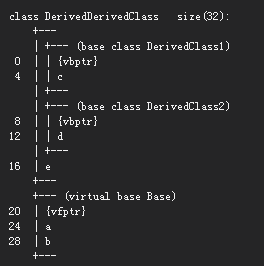
\includegraphics[scale = 0.8]{virtualDerivedDerivedVirutal.png}
					\caption{虚多继承-DD}
				\end{figure}
		
			\subparagraph{总结} \verb|->|
				
			\textbf{虚继承的作用是减少了对基类的重复,代价是增加了虚表指针的负担(更多的虚表指针)。}
			
			\textbf{如果是虚继承,那么子类会有两份虚指针},一份指向自己的虚表,另一份指向虚基表,多重继承时虚基表与虚基表指针有且只有一份
			
	\newpage		
	\section{ELF}
		\url{https://www.cnblogs.com/gtarcoder/p/6006023.html}	
		
		\url{http://www.cnblogs.com/xmphoenix/archive/2011/10/23/2221879.html}
\chapter{extern 关键字}
       
     \section{基本解释}extern可以置于变量或者函数前,以标示变量或者函数的定义在别的文件中,提示编译器遇到此变量和函数时在其他模块中寻找其定义
       
     \section{问题}
	     \subsubsection{作用范围-可见性的关键字}
	        \subparagraph{extern 变量}
		        该关键字告诉编译器,\textbf{其声明的函数和变量}\textit{可以}在本模块或其它模块中\textbf{使用}。
		        
		        在一个源文件里定义了一个数组:\verb|char a[6]|;
		         
		        在另外一个文件里用下列语句进行了声明:\verb|extern char *a|;
		        
		        请问,这样可以吗? 
		        
		        答案与分析:
		        
		        答:不可以,程序运行时会告诉你非法访问。原因在于,指向类型T的指针并不等价于类型T的数组。\verb|extern char *a|声明的是一个指针变量而不是字符数组,因此与实际的定义不同,从而造成运行时非法访问。应该将声明改为\verb|extern char a[ ]|。
		        
		        注意:{\color{blue}\textbf{你在*.c文件中声明了一个全局的变量,这个全局的变量如果要被引用,就放在*.h中并用extern来声明}}
		        
	      \subsubsection{连接申明linkage declaration}        
	        \subparagraph{extern"C"}
		        被\verb|extern "C"|修饰的变量和函数是\textbf{按照}\verb|C|语言方式\textbf{编译和连接的}
		        
		        在\verb|C++|环境下\textbf{使用}\verb|C|函数的时候,常常会出现编译器无法找到\verb|obj|模块中的\verb|C|函数定义,从而导致链接失败的情况,应该如何解决这种情况呢?
	        
		        答案与分析:
		        
		        \verb|C++|语言在编译的时候为了解决函数的多态问题,会将函数名和参数联合起来生成一个中间的函数名称,而\verb|C|语言则不会.
		        
		        因此会造成链接时找不到对应函数的情况,此时C函数就需要用\verb|extern "C"|进行链接指定,这告诉编译器,请保持我的名称,不要给我生成用于链接的中间函数名。
		        下面是一个标准的写法[函数的头文件--在.h文件]:
		        \begin{lstlisting}
	#ifdef __cplusplus
	#if __cplusplus
		extern "C"{
	#endif
	#endif /* __cplusplus */ 
	
	/*
	*
	*  defined  what u use
	*
	*/
	
	#ifdef __cplusplus
	#if __cplusplus
		}
	#endif
	#endif /* __cplusplus */ 	        
		        \end{lstlisting}
        
	        \subparagraph{extern 函数声明} 当函数提供方单方面修改函数原型时,如果使用方不知情继续沿用原来的\verb|extern|申明,这样编译时编译器不会报错。但是在运行过程中,因为少了或者多了输入参数,往往会照成系统错误,这种情况应该如何解决?
	        
	        答案与分析:
	        
	        目前业界针对这种情况的处理没有一个很完美的方案,\textbf{通常的做法是提供方在自己的}\verb|xxx_pub.h|\textbf{中提供对外部接口的声明},然后调用方\verb|include|该头文件,从而省去\verb|extern|这一步。以避免这种错误。
	        宝剑有双锋,对\verb|extern|的应用,不同的场合应该选择不同的做法。
	      
\chapter{volatile 关键字}
	\section{含义}
		\begin{enumerate}
			\item \textbf{不会在两个操作之间把volatile变量缓存在寄存器中}。在多任务、中断、甚至setjmp环境下,变量可能被其他的程序改变,编译器自己无法知道,volatile就是告诉编译器这种情况。
			\item \textbf{不做常量合并}、常量传播等优化
			\item \textbf{对volatile变量的读写不会被优化掉}。如果你对一个变量赋值但后面没用到,编译器常常可以省略那个赋值操作,然而对Memory Mapped IO的处理是不能这样优化的。
		\end{enumerate}
			  
		\url{http://www.cnblogs.com/yc_sunniwell/archive/2010/06/24/1764231.html}     
\chapter{explicit 关键字}

	\section{作用}
			explicit关键字用来修饰类的构造函数,被修饰的构造函数的类,\textbf{不能发生}相应的\textbf{隐式类型转换-根据构造函数},\textbf{只能以显示的方式}进行\textbf{类型转换}。
        
	        explicit 关键字作用于单个参数的构造函数。
	        \subparagraph{示例}:
		        \begin{lstlisting}
	/////////未加explicit时的隐式类型转换/////////////
	class Circle 
	{ 
	public: 
		Circle(double r) : R(r) {} 
		Circle(int x, int y = 0) : X(x), Y(y) {} 
		Circle(const Circle& c) : R(c.R), X(c.X), Y(c.Y) {} 
	private: 
		double R; 
		int    X; 
		int    Y; 
	}; 
	
	int _tmain(int argc, _TCHAR* argv[]) 
	{ 
		//发生隐式类型转换 
		//编译器会将它变成如下代码 
		//tmp = Circle(1.23) 
		//Circle A(tmp); 
		//tmp.~Circle(); 
		Circle A = 1.23;  
		//注意是int型的,调用的是Circle(int x, int y = 0) 
		//它虽然有2个参数,但后一个有默认值,任然能发生隐式转换 
		Circle B = 123; 
		//这个算隐式调用了拷贝构造函数 
		Circle C = A; 
		
		return 0; 
	} 
	
	
	
	/////////加了explicit关键字后,可防止以上隐式类型转换发生//////////
	
	class Circle 
	{ 
	public: 
		explicit Circle(double r) : R(r) {} 
		explicit Circle(int x, int y = 0) : X(x), Y(y) {} 
		explicit Circle(const Circle& c) : R(c.R), X(c.X), Y(c.Y) {} 
	private: 
		double R; 
		int    X; 
		int    Y; 
	};  
	int _tmain(int argc, _TCHAR* argv[]) 
	{ 
		//一下3句,都会报错 
		//Circle A = 1.23;  
		//Circle B = 123; 
		//Circle C = A; 
		
		//只能用显示的方式调用了 
		//未给拷贝构造函数加explicit之前可以这样 
		Circle A = Circle(1.23); 
		Circle B = Circle(123); 
		Circle C = A; 
		
		//给拷贝构造函数加了explicit后只能这样了 
		Circle A(1.23); 
		Circle B(123); 
		Circle C(A); 
		return 0; 
	} 		        	
		        \end{lstlisting}
\chapter{friend 关键字}
\section{目的}
		    采用类的机制后实现了数据的隐藏与封装,\textbf{只有}类的成员函数才能访问类的私有成员,程序中的其他函数是无法访问私有成员的。
	        
	        非成员函数可以访问类中的公有成员,但是如果将数据成员都定义为公有的,这又破坏了隐藏的特性。另外,应该看到在某些情况下,\textbf{需要频繁地访问类的数据成员,特别是在对某些成员函数多次调用时,由于参数传递,类型检查和安全性检查等都需要时间开销,而影响程序的运行效率}。这时可以将这些函数定义为该函数的友元函数
        
		    \textbf{友元函数是可以直接访问类的私有成员的非成员函数。它是定义在类外的普通函数,但需要在类的定义中加以声明},声明时只需在友元的名称前加上关键字\verb|friend|
		    
\section{友元函数}
		    \begin{lstlisting}
	class CPoint
	{
	public:
		CPoint();
		CPoint(double _x, double _y){ x = _x; y=_y;}
		friend double calcDistance(CPoint& pt1, CPoint& pt2);
	private:
		double x;
		double y;
	};
	
	double calcDistance(CPoint& pt1, CPoint& pt2)
	{
		double dx = pt1.x - pt2.x;
		double dy = pt1.x - pt2.x;
		return sqrt(dx*dx+dy*dy);
	}
	
	int main(int argc, char* argv[])
	{
		CPoint pt1(3.0, 4.0);
		CPoint pt2(4.0, 8.0);
		double dist = calcDistance(pt1, pt2);
		cout<<"calcDistance(pt1, pt2)="<<dist<<endl;
		getchar();
		return 1;
	}		    
		    \end{lstlisting}
		    
\section{友元类}
			    当一个类作为另一个类的友元时,这就意味着这个类的所有成员函数都是另一个类的友元函数
		    
		    \subparagraph{例子}:
			    在感情生活中,我们经常会遇到一些霸道的对象说:你的就是我的,我的就是我的(\verb|need is word ,word is still word|)!,你有多少异性朋友,不能\verb|private|,你银行卡的密码、\verb|QQ|密码需要不能\verb|private|,即使\verb|private|了,也要让我知道。呵呵,当然,对于一些大爱无私的男的,也总会满足自己女友的一些霸道条款。为了说明友元类,看下例
		    
		     \begin{lstlisting}
	class CBoyFriend
	{
	public:
		CBoyFriend():girl_number(10),qq_password("123456789"){}
		friend class CGirlFriend;
	
	private:
		int howManyGirlFriends(){ return girl_number;}	
		string whenToBuyRoses(){ return string("everyNight");}
	private:
		string bank_card;
		string bank_card_password;
		string qq_id;
		string qq_password;	
		int girl_number;
	};
	
	class CGirlFriend
	{
	public:
		CGirlFriend(){};
		CBoyFriend boy;
		void printBoyFriend()
		{
			cout<<"bank_card:"<<boy.bank_card<<endl;
			cout<<"password:"<<boy.bank_card_password<<endl;
			cout<<"qq_id:"<<boy.qq_id<<endl;
			cout<<"qq_password:"<<boy.qq_password<<endl;
		}
	};
	
	
	int main(int argc, char* argv[])
	{	
		CGirlFriend girl;	
		girl.printBoyFriend();
		
		getchar();
		return 1;
	}		     
		    \end{lstlisting}
		    
		    \begin{enumerate}[fullwidth,itemindent = 2em,label=(\arabic*)]
		    	\item 友元函数不能被继承
		    	\item 友元关系是单向的,不具有交换性。若类B是类A的友元,类A不一定是类B的友元,要看在类中是否有相应的声明
		    	\item 友元关系不具有传递性。若类B是类A的友元,类C是B的友元,类C不一定是类A的友元
		    \end{enumerate}
		    
		    
		    
\chapter{mutable 关键字}
\section{目的}
	mutalbe的中文意思是“可变的,易变的”,跟constant(既C++中的const)是反义词。
	
	在C++中,mutable也是为了突破const的限制而设置的。被mutable修饰的变量,将永远处于可变的状态,即使在一个const函数中。
	
	我们知道,如果类的成员函数不会改变对象的状态,那么这个成员函数一般会声明成const的。但是,\textbf{有些时候,我们需要在const的函数里面修改一些跟类状态无关的数据成员},那么这个数据成员就应该被mutalbe来修饰。
\section{示例}
	\begin{lstlisting}
	class ClxTest
	{
	public:
		ClxTest();
		~ClxTest();
		
		void Output() const;
		int GetOutputTimes() const;
	
	private:
		mutable int m_iTimes;
	};
	
	ClxTest::ClxTest()
	{
		m_iTimes = 0;
	}
	
	ClxTest::~ClxTest(){}
	
	// const 函数修改与类状态无关的数据成员
	void ClxTest::Output() const
	{
		cout << "Output for test!" << endl;
		m_iTimes++;
	}
	
	int ClxTest::GetOutputTimes() const
	{
		return m_iTimes;
	}
	
	void OutputTest(const ClxTest& lx)
	{
		cout << lx.GetOutputTimes() << endl;
		lx.Output();
		cout << lx.GetOutputTimes() << endl;
	}	
	\end{lstlisting}

\chapter{类型转换}
\section{static\_cast}
	\verb|static_cast|:基本拥有与C旧式转型相同的威力与意义,以及相同的限制。它用的最多,\textbf{主要是在基本类型之间的转换}
	\begin{lstlisting}
	void test1()   
	{     
		int first=23,second=31;   
		double res=(double)first/second; //旧式C语法   
		double res2=static_cast<double>(first)/second;//新式C++转型符   
		cout<<res<<" "<<res2<<endl;// 0.741935 0.741935   
		//  char* str="789";   
		//  cout<<static_cast<int>(str)<<endl;//error:无法从char*转换为int   
	}  
	\end{lstlisting}
\section{const\_cast}
	\verb|const_cast|:用来\textbf{去掉表达式中的常量性(constness)},常量属性多体现在指针和引用,因为如果没有指针和引用,就不存在不小心修改了不能修改的数据
	
\section{dynamic\_cast}
	\verb|dynamic_cast|:用来执行继承体系中“\textbf{安全的向下转型或跨系转型动作}“,就是父类对象指针转化为子类对象指针。可以利用\verb|dynamic_cast|将指向base classObject的pointer或reference转型为指向derived classObject的pointer或reference,如果转型失败,会以一个null指针(转换的是pointer的话)或一个exception表现出来(转换的是reference的话)
	
	\begin{lstlisting}
	class B
	{
	public:
		virtual void fun()
		{
			cout<<"B.fun()"<<endl;
		}
	};   
	
	class D1:public B
	{
	public:
		void fun()
		{
			cout<<"D1.fun()"<<endl;
		}
		void fun2()
		{
			cout<<"D1.fun2()"<<endl;
		}
	};   

	class CBase{};
	 
	class CDerived : public CBase{};
	
	void test3()   
	{    
		// 父类指针转换为子类指针时,父类要有虚函数
		B* pb=new D1();   
		D1* pd1=dynamic_cast<D1*>(pb);
		
		// 子类指针转换为父类指针,不需要虚函数
		CDerived dc;   
		CDerived* dp=&dc;   
		CBase* cc1=dp;// 老式:子类指针转换为父类指针,即父类指针指向子类对象   
		CBase* cb1=dynamic_cast<CBase*>(dp);// 使用dynamic_cast将指向继承类的指针转化为指向基类的指针   
		printf("point: %d, %d, %d, %d",dp,cc1,cb1,&dc);// 它们的地址相同,说明它们在内存中是同一个地址;即子类指针转换为父类指针,父类的地址指向子类的地址,且是相同的。   
		
		CBase& cc2=dc;   
		CBase& cb2=dynamic_cast<CBase&>(dc);// 使用dynamic_cast将指向继承类的引用转化为指向基类的引用   
	}
	\end{lstlisting} 
\section{reinterpret\_cast}
		\url{http://www.cnblogs.com/ider/archive/2011/07/30/cpp_cast_operator_part3.html}
		
		\verb|reinterpret_cast <new_type> (expression)|
		
		\verb|reinterpret_cast|运算符是用来处理无关类型之间的转换;它会产生一个新的值,这个值会有与原始参数(expressoin)有完全相同的比特位。

		\verb|reinterpret_cast|可以,或者说应该在什么地方用来作为转换运算符:
		\begin{itemize}
			\item 从\textbf{指针}类型到一个足够大的整数类型
			\item 从整数类型或者枚举类型到\textbf{指针}类型
			\item 从一个指向函数的\textbf{指针}到另一个\textbf{不同类型}的指向函数的\textbf{指针}
			\item 从一个指向对象的\textbf{指针}到另一个\textbf{不同类型}的指向对象的\textbf{指针}
			\item 从一个指向类函数成员的\textbf{指针}到另一个指向\textbf{不同类型}的函数成员的\textbf{指针}
			\item 从一个指向类数据成员的\textbf{指针}到另一个指向\textbf{不同类型}的数据成员的\textbf{指针}
		\end{itemize}
		
		所以总结来说:\verb|reinterpret_cast|用在\textbf{任意指针(或引用)类型之间的转换};以及\textbf{指针与足够大的整数类型之间的转换};从\textbf{整数类型(包括枚举类型)到指针类型},无视大小。
		
		\color{green}(所谓"足够大的整数类型",取决于操作系统的参数,如果是32位的操作系统,就需要整形(int)以上的;如果是64位的操作系统,则至少需要长整形(long)。具体大小可以通过sizeof运算符来查看)。\color{black}
\chapter{static\_assert 关键字}
\section{简介}
	其语法很简单:\verb|static_assert|(常量表达式,提示字符串)。
	
	如果第一个参数常量表达式的值为真(true或者非零值),那么\verb|static_assert|不做任何事情,就像它不存在一样,否则会产生一条编译错误,错误位置就是该\verb|static_assert|语句所在行,错误提示就是第二个参数提示字符串。
	
\section{说明}
	\begin{itemize}
		\item 使用\verb|static_assert|,我们可以在编译期间发现更多的错误,用编译器来强制保证一些契约,并帮助我们改善编译信息的可读性,尤其是用于模板的时候
		\item \verb|static_assert|可以用在全局作用域中,命名空间中,类作用域中,函数作用域中,几乎可以不受限制的使用
		\item 编译器在遇到一个\verb|static_assert|语句时,通常立刻将其第一个参数作为常量表达式进行演算,但如果该常量表达式依赖于某些模板参数,则延迟到模板实例化时再进行演算,这就让检查模板参数成为了可能
		\item 性能方面,由于是\verb|static_assert|编译期间断言,不生成目标代码,因此\verb|static_assert|不会造成任何运行期性能损失
	\end{itemize}
\section{范例}
	\begin{lstlisting}
	// 下面是一个来自MSDN的简单范例:该static_assert用来确保编译仅在32位的平台上进行,不支持64位的平台,该语句可以放在文件的开头处,这样可以尽早检查,以节省失败情况下的编译时间
	static_assert(sizeof(void *) == 4, "64-bit code generation is not supported.");
	
	
	 struct MyClass
	 {
	     char m_value;
	 };
	  
	 struct MyEmptyClass
	 {
	     void func();
	 };
	  
	 // 确保MyEmptyClass是一个空类(没有任何非静态成员变量,也没有虚函数)
	 static_assert(std::is_empty<MyEmptyClass>::value, "empty class needed");
	  
	 //确保MyClass是一个非空类
	 static_assert(!std::is_empty<MyClass>::value, "non-empty class needed");
	  
	 template <typename T, typename U, typename V>
	 class MyTemplate
	 {
	     // 确保模板参数T是一个非空类
	     static_assert(
	         !std::is_empty<T>::value,
	         "T should be n non-empty class"
	         );
	  
	     // 确保模板参数U是一个空类
	     static_assert(
	         std::is_empty<U>::value,
	         "U should be an empty class"
	         );
	  
	     // 确保模板参数V是从std::allocator<T>直接或间接派生而来,
	     // 或者V就是std::allocator<T>
	     static_assert(
	         std::is_base_of<std::allocator<T>, V>::value,
	         "V should inherit from std::allocator<T>"
	         );
  
	 };
	  
	 // 仅当模板实例化时,MyTemplate里面的那三个static_assert才会真正被演算,
	 // 藉此检查模板参数是否符合期望
	 // template class MyTemplate<MyClass, MyEmptyClass, std::allocator<MyClass>>;
	//通过这个例子我们可以看出来,static_assert可以很灵活的使用,通过构造适当的常量表达式,我们可以检查很多东西。比如范例中std::is_empty和std::is_base_of都是C++新的标准库提供的type traits模板,我们使用这些模板可以检查很多类型信息。
	\end{lstlisting}

\section{参考}
	\url{http://www.cnblogs.com/lvdongjie/p/4489835.html}
\chapter{命名空间}
\section{namespace 别名}\verb|namespace  BieMing = nameSpace'sName|
		   
\section{namespace 扩充}\verb|namespace  sameName{}|
	   
		   \subparagraph{例子}:
		   
		   \begin{lstlisting}
	namespace runrunrunrun
	{
		int a(10);
		char *str("gogogo");
		namespace run   //namespace's QianTao
		{
			int a(9);
		}
	}
	
	namespace runrunrunrun  //namespace's Expand
	{
		int  y(5);
		//int  a(15);Redefine error
	}
	
	namespace r = runrunrunrun;//namespace's aliaName
	
	void main132()
	{
		std::cout << r::run::a << std::endl;//namespace can QianTao
		std::cout << r::y << std::endl;
		std::cout << r::a << std::endl;
	}		   	
		   \end{lstlisting}
\chapter{引用}
	\section{引用 创建时 必须初始化}
		   
		   \verb|DataType &  Value(referenceValue);| 
		    
		    \verb|DataType &  Value = referenceValue;|
	    
	\section{引用不能重定义}即一旦定义,不能再重新指向别的变量。
	       
	       一旦一个引用被初始化为指向一个对象,它就不能改变为另一个对象的引用,指针则可以在任何时候指向另一个对象。
	\section{函数中的引用}
	       
	       \begin{lstlisting}
	int* f(int* X)
	{
		(*X)++;
		return X; //Safe, X is outside this scope
	}
	
	int& g(int& x)
	{
		x++;// Same effectas in f()
		return x;// Safe, outside this scope
	}
	
	int& h()
	{
		int q;
		//return q; //Error, Because in the Stack Memery,Then we can only use once. if we use the pointer, Then if we save the address,Then we can use too,but not Safe at all. See Example 3.1
		static int x;
		return x; //Safe, x lives outside this scope.
	}
	
	//Reference TO Pointer
	void func(int* &i)
	{
		i++;// change the int* pointer's address, not the value i.
	}		       	
	       \end{lstlisting}
	       
	       \subparagraph{例子3.1}:
	       
		       \begin{lstlisting}
	int& funcTest()
	{
		int test = 10;
		return test;
	}
	
	int main()
	{
		int& T = funcTest();
		/*if change to (int T) Then can work,
		Because we can catch when the top temp local value pop out(Stack), 
		if such reference do not same the second. 
		Because the refer first is a Temp Local Register value.
		second the Memory has been recalled ,so it is a gabash value.
		
		Heap:the C++ do not allow use the memory that have been deleted.
		
		int* p = new int;
		delete p;
		
		cout << p <<endl;  That not allow
		*/
		
		cout << T<<endl;
		cout << T<<endl;
		return 0;
	}		       	
		       \end{lstlisting}
   
	\section{引用 右值} 两个\verb|&|, 即引用CPU的寄存器中的值 或 内存中的值
			\subparagraph{参考网址}\url{http://www.cnblogs.com/qicosmos/p/4283455.html}
			
			\subparagraph{右值引用的声明期限}getVar()产生的临时值不会在表达式结束之后就销毁了,而是会被“续命”,他的生命周期将会通过右值引用得以延续,和变量k的声明周期一样长
				\begin{lstlisting}
	T&& k = getVar();
				\end{lstlisting}
				
			\subparagraph{类型不确定性}仅仅是当发生自动类型推导(如函数模板的类型自动推导,或auto关键字)的时候,\verb|T&&|才是universal references
			
			\subparagraph{完美转发}在函数模板中,完全依照模板的参数的类型(即保持参数的左值、右值特征),将参数传递给函数模板中调用的另外一个函数
	   
\chapter{enum 的使用}

	\section{定义}
		    \verb|enum color:char{ red='A' , yellow, green, white };|
		    
		    \verb|enum class Enum2 : unsigned int {Val1, Val2};|
		    
		    \verb|enum Enum3 : unsigned long {Val1 = 1, Val2};|
		    
		    \begin{itemize}
		    	\item 可以指定存储类型
		    	\item 可以指定存储值的开始,默认为0(int,char都是),本例为‘A’,则yellow 为B,...
		    \end{itemize}
		
	\section{使用}
		\subsection{类外函数}
			\verb|color mycolor = red;|
			
			//mycolor = 'A';//确保在枚举的范围的之内不出错,枚举不可以当成基本数据类型使用
			
			\verb|mycolor = color::white|;//新语法
			
			\verb|color mycolor1(red);|
			
			\verb|color mycolor2(color::red);|
		
		\subsection{类中}
			\begin{lstlisting}
	class SpreadsheetCell
	{
	public:
		// Omitted for brevity
		enum class Colors { Red = 1, Green, Blue, Yellow };
		void setColor(Colors color);
	private:
		// Omitted for brevity
		Colors mColor = Colors::Red;
	};
	
	void SpreadsheetCell::setColor(Colors color)
	{
		mColor = color;
	}
	
	SpreadsheetCell myCell(5);
	myCell.setColor(SpreadsheetCell::Colors::Blue);
			\end{lstlisting}
	\section{注意事项}
		\begin{lstlisting}
	enum Enum1;                      // Illegal in C++03 and C++11; the underlying type cannot be determined.
	enum Enum2 : unsigned int;       // Legal in C++11, the underlying type is specified explicitly.
	enum class Enum3;                // Legal in C++11, the underlying type is int.
	enum class Enum4 : unsigned int; // Legal in C++11.
	enum Enum2 : unsigned short;     // Illegal in C++11, because Enum2 was formerly declared with a different underlying type.		
		\end{lstlisting}
\chapter{模版}
	参考C++\_STL 中的泛型编程一章。
	
\chapter{异常}
	
		
\chapter{编译}
	\section{Windows-VisualStudio}
		\subsection{配置全局VC++目录}
			\begin{enumerate}
				\item  随便打开一个项目,然后点击菜单中的 \verb|视图->其他窗口->属性管理器|
				
				\item  打开属性管理器,点击项目前的箭头,展开项目,找到\verb|Debug|或者\verb|Release| 下面的 \verb|Microsoft.Cpp| \verb|.Win32.user| 这个属性
				
				\item  双击会出现一个跟在项目上右键属性一样的窗口,修改里面的“\verb|VC++目录|”就是修改了全局的,
			\end{enumerate}
		\subsection{配置第三方程序库-以opencv 示例}
			\subsubsection{下载配置所需}
				\subparagraph{1.VisualStudio2010}
				\subparagraph{2.OpenCV2.4.8}
			
			\subsubsection{安装}
				\subparagraph{1.安装位置不影响}
				\subparagraph{2.配置Path系统环境}	
				  \verb|PATH|是路径的意思,\verb|PATH|环境变量中存放的值,就是一连串的路径。不同的路径之间,用英文的分号(;)分隔开。\textbf{系统执行用户命令时,若用户未给出绝对路径,则首先在当前目录下寻找相应的可执行文件、批处理文件(另外一种可以执行的文件)等}。若找不到,再依次在\verb|PATH|保存的这些路径中寻找相应的可执行的程序文件。系统就以第一次找到的为准;若搜寻完PATH保存的所有路径都未找到,则会显示类似于\textbf{"找不到该命令"}的错误信息。
			
			\subsubsection{配置}
				\subparagraph{1.Create Project}建立一个VisualStudio  ConsoleApplication Empty Project
				\subparagraph{2.配置}
				\begin{itemize}[itemindent = 2em]
					\item -右键项目
					\item -Properties
					\item -VC++ Directories
					\item -配置include Directories += 安装目录$ \verb|\|$opencv$ \verb|\|$build$ \verb|\|$include; += 安装目录$ \verb|\|$ opencv$ \verb|\|$build$ \verb|\|$include$ \verb|\|$opencv; +=安装目录$ \verb|\|$opencv$ \verb|\|$build$ \verb|\|$include$ \verb|\|$opencv2;
					\item -配置Liberary Directories += 安装目录$ \verb|\|$opencv$ \verb|\|$build$ \verb|\|$x86$ \verb|\|$vc10$ \verb|\|$lib;
					\item -Linker选项 -input
					\item Additional Dependecies 添加如下库:见参考文献
				\end{itemize}
			
			\subsubsection{编程测试}注意:路径中的单杠要换成双杠\verb|\\|
			
		\subsection{dll 与 lib 的配置}
			\subparagraph{静态lib}它将\textbf{导出声明和实现均放到lib中},编译后所有代码都嵌入到宿主程序中去。
			\subparagraph{动态lib}相当于一个h文件,它是\textbf{对实现部分(.DLL)的导出部分的声明}。编译后只是将导出声明部分编译到宿主程序中,\textbf{运行时需要相应的DLL文件的支持,否则无法工作}。当生成一个新的DLL时,也会有配套的lib产生(即二者需一起分发),此时的lib即为动态lib-->\textbf{[如openGL-glut 工具库]}
			
			动态库的\textbf{2种配置方法}:
				\begin{enumerate}[itemindent = 2em]
					\item 需把对应的 .dll 文件以及.lib 文件和.h文件(结合方式时)拷贝至调用的程序目录下
					\item 在visual studio 中把c++目录的include 目录 和 附属lib 目录配置好后,再把对应的.dll 文件考到系统的 system32 或 sysWOW64 中..这样的好处是,一劳永逸。 不过可能你并没有权限操作执行复制操作..此时参考下文。
				\end{enumerate}
		
		\subsection{常见错误}
			\subsubsection{}	
			\subparagraph{参考}
			dll与lib:\url{http://blog.csdn.net/heyabo/article/details/8721611}
			
			win10 权限更改:\url{http://blog.163.com/qywwkai@126/blog/static/21003042201541235335362/}
	\section{Linux - Makefile}
	
			\url{http://blog.csdn.net/haoel/article/details/2887/}
		\subsection{Makefile 规则}
			\begin{lstlisting}
	target ... : prerequisites ...
		command
		...
		...
			\end{lstlisting}
			
			\begin{itemize}
				\item \verb|target| 就是一个目标文件,可以是\verb|Object File|,也可以是\verb|执行文件|,当然也可以是个标签(clean)
				\item \verb|prerequisites| 就是要生成那个\verb|target|所需要的\verb|文件|或是\verb|目标|
				\item \verb|command| 就是\verb|make|需要执行的命令-任意的\verb|Shell命令|
			\end{itemize}
			
			\subsubsection{示例}
				\begin{lstlisting}
	edit :  main.o kbd.o command.o display.o /
			insert.o search.o files.o utils.o
		cc -o edit main.o kbd.o command.o display.o /
					insert.o search.o files.o utils.o
	main.o : main.c defs.h
		cc -c main.c
	kbd.o : kbd.c defs.h command.h
		cc -c kbd.c
		
		...
		
	utils.o : utils.c defs.h
		cc -c utils.c
	clean :
		rm edit main.o kbd.o command.o display.o /
		insert.o search.o files.o utils.o
				\end{lstlisting}
				\begin{itemize}
					\item 在定义好依赖关系后,\textbf{后续的那一行}定义了如何生成目标文件的操作系统命令,\textbf{一定要以一个Tab键作为开头}。
					\item \verb|反斜杠(/)|是\textbf{换行符}的意思
				\end{itemize}
		
		\subsection{make 执行流程}
			\begin{enumerate}
				\item \verb|make|会在当前目录下找名字叫“\verb|Makefile|”或“\verb|makefile|”的文件
				\item 如果找到,它会找文件中的第一个目标文件(\verb|target|),在上面的例子中,他会找到“\verb|edit|”这个文件,并把这个文件作为最终的目标文件。
				\item 如果\verb|edit|文件不存在,或是edit所依赖的后面的 \verb|.o|文件的文件修改时间要比\verb|edit|这个文件新,那么,他就会执行后面所定义的命令来生成\verb|edit|这个文件
				\item 如果\verb|edit|所依赖的\verb|.o|文件也存在,那么\verb|make|会在当前文件中找目标为\verb|.o|文件的依赖性,如果找到则再根据那一个规则生成\verb|.o|文件
				\item 当然,你的\verb|C|文件和\verb|H|文件是存在的啦,于是\verb|make|会生成 \verb|.o| 文件,然后再用 \verb|.o |文件生命\verb|make|的终极任务,也就是执行文件\verb|edit|了
			\end{enumerate}
			
		\subsection{makefile 中使用变量}
			\begin{lstlisting}
	objects = main.o kbd.o command.o display.o /
		insert.o search.o files.o utils.o
	edit : $(objects)
		cc -o edit $(objects)
			\end{lstlisting}
		
		\subsection{make 的自动推倒}
			只要、ver看到一个\verb|[.o]文件|,它就会自动的把\verb|[.c]文件|加在依赖关系中,如果\verb|make|找到一个\verb|whatever.o|,那么\verb|whatever.c|,就会是\verb|whatever.o|的依赖文件。并且 \verb|cc -c whatever.c |也会被推导出来
			
			于是,我们的\verb|makefile|再也不用写得这么复杂。我们的是新的\verb|makefile|又出炉了。
			\begin{lstlisting}
	objects = main.o kbd.o command.o display.o /
		insert.o search.o files.o utils.o
		
	edit : $(objects)
		cc -o edit $(objects)
		
	main.o : defs.h
	kbd.o : defs.h command.h
	command.o : defs.h command.h
	display.o : defs.h buffer.h
	insert.o : defs.h buffer.h
	search.o : defs.h buffer.h
	files.o : defs.h buffer.h command.h
	utils.o : defs.h
	
	.PHONY : clean
	clean :
		rm edit $(objects)
			\end{lstlisting}
			
			\subparagraph{进一步自动化}即然我们的\verb|make|可以自动推导命令,那么我看到那堆\verb|[.o]和[.h]|的依赖就有点不爽,那么多的重复的\verb|[.h]|,\textbf{能不能}把其\textbf{收拢起来},好吧,没有问题,这个对于\verb|make|来说很容易,谁叫它提供了自动推导命令和文件的功能呢?来看看最新风格的\verb|makefile|吧。
			
				\begin{lstlisting}
	objects = main.o kbd.o command.o display.o /
		insert.o search.o files.o utils.o
		
	edit : $(objects)
		cc -o edit $(objects)
		
	$(objects) : defs.h
	kbd.o command.o files.o : command.h
	display.o insert.o search.o files.o : buffer.h
	
	.PHONY : clean
	clean :
		rm edit $(objects)
				\end{lstlisting}
		\subsection{添加依赖库}
		
			大牛文章\url{http://blog.csdn.net/qq_33850438/article/details/52014399}	
		\subsection{代码泄漏检测}
			\url{http://blog.csdn.net/21aspnet/article/details/8172124}
			
		\subsection{参考文献}
		
			makefile :\url{http://blog.csdn.net/liang13664759/article/details/1771246/}
			
			\url{http://blog.csdn.net/xzz_hust/article/details/8879569}

\chapter{调试}			
	\section{Linux - 调试 GDB}
		\subsection{使用 GDB}
			\paragraph{-g 编译项目}
				一般来说\verb|GDB|主要调试的是\verb|C/C++|的程序。要调试\verb|C/C++|的程序,首先在编译时,我们\textbf{必须要把调试信息加到可执行文件中}。使用编译器\verb|(cc/gcc/g++)|的\verb| -g |参数可以做到这一点。如:
				
				>\verb| cc -g hello.c -o hello|
				
				>\verb| g++ -g hello.cpp -o hello|
				
			\paragraph{启动 GDB}
				成功编译目标代码以后,让我们来看看如何用\verb|gdb|来调试他
				
				\verb|gdb <program>| (\verb|program|就是你的\textbf{执行文件},不是\verb|.c .cpp .o|, 而是加\verb|-g| 编译后的\verb|hello|)
				
			
			\paragraph{GDB 常用 命令}
				\subparagraph{基础 命令}
					 \begin{itemize}[itemindent = 1em]
					 	\item \verb|n |单条语句执行,\verb|next|命令简写
					 	\item \verb|r |运行程序,\verb|run|命令简写
					 	\item \verb|c |继续运行程序,\verb|continue|命令简写
					 	\item \verb|p i |打印变量\verb|i|的值,\verb|print|命令简写
					 	\item \verb|finish |退出函数
					 	\item \textbf{设置断点}:我们用\verb|break|命令来设置断点。正面有几点设置断点的方法:
					 	
						 	\begin{enumerate}
						 		\item \verb|break <function> | :在进入指定函数时停住。\verb|C++|中可以使用\verb|class::function|或\verb|function(type,type)|格式来指定函数名
						 		\item \verb|break <linenum> |:在指定行号停住
						 		\item \verb|break +offset, 	break -offset|:在当前行号的前面或后面的\verb|offset |行停住。\verb|offiset |为自然数
						 		\item \verb|break ... if <condition>|: \verb|...|可以是上述的参数,\verb|condition|表示条件,在条件成立时停住。比如在循环境体中,可以设置\verb|break if i=100|,表示当\verb|i为100|时停住程序
						 		\item \verb|break *address |在程序运行的内存地址处停住
						 		\item 查看断点时,可使用\verb|info|命令: \verb|info breakpoints [n], info break [n]|注:\verb|n|表示断点号
						 	\end{enumerate}
					 	\item \textbf{观察点}:观察点一般来观察某个表达式(变量也是一种表达式)的值是否有变化了,如果有变化,马上停住程序。我们有下面的几种方法来设置观察点:
						 	\begin{enumerate}
						 		\item \verb|watch <expr> |:为表达式(变量)\verb|expr|设置一个观察点。\textbf{一量表达式值有变化时},马上停住程序
						 		\item \verb|rwatch <expr>|:当表达式(变量)\verb|expr|\textbf{被读时},停住程序
						 		\item \verb|awatch <expr>|:当表达式(变量)的值\textbf{被读或被写时},停住程序
						 		\item \verb|info watchpoints|:列出当前所设置了的所有观察点
						 	\end{enumerate}
					 	\item \textbf{捕捉点}:你可设置捕捉点来补捉程序运行时的一些事件。如:载入共享库(动态链接库)或是\verb|C++|的异常。设置捕捉点的格式为:
					 	
						 	\verb|catch <event>| 当event发生时,停住程序。event可以是下面的内容:
						 	
						 	\begin{enumerate}
						 		\item \verb|throw| 一个C++抛出的异常。(\verb|throw|为关键字)
						 		\item \verb|catch| 一个C++捕捉到的异常。(\verb|catch|为关键字)
						 		\item \verb|exec| 调用系统调用\verb|exec|时。(\verb|exec|为关键字,目前此功能只在HP-UX下有用)
						 		\item \verb|fork| 调用系统调用\verb|fork|时。(\verb|fork|为关键字,目前此功能只在HP-UX下有用)
						 		\item \verb|vfork| 调用系统调用\verb|vfork|时。(\verb|vfork|为关键字,目前此功能只在HP-UX下有用)
						 		\item \verb|load| 或 \verb|load <libname>| 载入共享库(动态链接库)时。(\verb|load|为关键字,目前此功能只在HP-UX下有用)
						 		
						 		\item \verb|unload| 或 \verb|unload <libname>| 卸载共享库(动态链接库)时。(\verb|unload|为关键字,目前此功能只在HP-UX下有用)
						 	\end{enumerate}
						 	
						 	\verb|tcatch <event> |
						 	
						 	只设置一次捕捉点,当程序停住以后,应点被自动删除。
					 \end{itemize}
				\subparagraph{Help 命令}启动\verb|gdb|后,就你被带入\verb|gdb|的调试环境中,就可以使用\verb|gdb|的命令开始调试程序了,\verb|gdb|的命令可以使用\verb|help|命令来查看,如下所示
				
				\begin{lstlisting}
	/home/hchen> gdb
	GNU gdb 5.1.1
	Copyright 2002 Free Software Foundation, Inc.
	GDB is free software, covered by the GNU General Public License, and you are
	welcome to change it and/or distribute copies of it under certain conditions.
	Type "show copying" to see the conditions.
	There is absolutely no warranty for GDB.  Type "show warranty" for details.
	This GDB was configured as "i386-suse-Linux".
	(gdb) help
	List of classes of commands:
	aliases -- Aliases of other commands
	breakpoints -- Making program stop at certain points
	data -- Examining data
	files -- Specifying and examining files
	internals -- Maintenance commands
	obscure -- Obscure features
	running -- Running the program
	stack -- Examining the stack
	status -- Status inquiries
	support -- Support facilities
	tracepoints -- Tracing of program execution without stopping the program
	user-defined -- User-defined commands
	Type "help" followed by a class name for a list of commands in that class.
	Type "help" followed by command name for full documentation.
	Command name abbreviations are allowed if unambiguous.
	(gdb)	
				\end{lstlisting}
				
			 \verb|gdb|的命令很多,\verb|gdb|把之分成许多个种类。\verb|help|命令只是例出\verb|gdb|的命令种类,如果要看种类中的命令,可以使用\verb|help <class>| 命令,如:\verb|help breakpoints|,查看设置断点的所有命令。也可以直接\verb|help <command>|来查看命令的帮助
		\subsection{参考}
			基本使用:\url{http://www.cnblogs.com/kunhu/p/3603268.html}
			
			大牛教程博客-1:\url{http://blog.csdn.net/haoel/article/details/2879}
			
			大牛教程博客-2:\url{http://blog.csdn.net/haoel/article/details/2880}
			
			大牛教程博客-3:\url{http://blog.csdn.net/haoel/article/details/2881}
			
			大牛教程博客-4:\url{http://blog.csdn.net/haoel/article/details/2882}
			
			大牛教程博客-5:\url{http://blog.csdn.net/haoel/article/details/2883}
			
			大牛教程博客-6:\url{http://blog.csdn.net/haoel/article/details/2884}
			
			大牛教程博客-7:\url{http://blog.csdn.net/haoel/article/details/2885}
\chapter{工程-细节}
\section{语言使用基本问题}
		\subsection{注释格式}
			\subsubsection{函数注释}
			\begin{lstlisting}
	/*
	* func()
	*
	* Description of the function.
	*
	* Parameters:
	* 	int param1: parameter 1.
	* Returns: int
	* 	An integer representing...
	* Throws:
	* 	Exception1 if...
	* Notes:
	* 	Additional notes...
	*/
			\end{lstlisting}
			\subsubsection{代码注释}
			\begin{lstlisting}
	/*
	* Implements the "insertion sort" algorithm. The algorithm separates the
	* array into two parts--the sorted part and the unsorted part. Each
	* element, starting at position 1, is examined. Everything earlier in the
	* array is in the sorted part, so the algorithm shifts each element over
	* until the correct position is found for the current element. When the
	* algorithm finishes with the last element, the entire array is sorted.
	*/
	void sort(int inArray[], int inSize)
	{
		// Start at position 1 and examine each element.
		for (int i = 1; i < inSize; i++) {
			// Invariant: All elements in the range 0 to i-1 (inclusive) are sorted.
			int element = inArray[i];
			// j marks the position in the sorted part of the array.
			int j = i – 1;
			// As long as the current slot in the sorted array is higher than
			// the element, shift the slot over and move backwards.
			while (j >= 0 && inArray[j] > element) {
				inArray[j+1] = inArray[j];
				j--;
			}
			// At this point the current position in the sorted array
			// is *not* greater than the element, so this is its new position.
			inArray[j+1] = element;
		}
	}
			\end{lstlisting}
		\subsection{预编译}
			\begin{lstlisting}
	单次编译
	#ifndef MYHEADER_H
	#define MYHEADER_H
	// ... the contents of this header file
	#endif
	
	If your compiler supports the #pragma once directive, and most modern compilers do, this can be
	rewritten as follows:
	#pragma once
	// ... the contents of this header file
	
	条件使用
	#ifdef [key]
	// ...
	#endif
			\end{lstlisting}
				
		\subsection{变量问题}
			\subsubsection{变量(包括成员)命名}
				\begin{figure}[h]
					\centering
					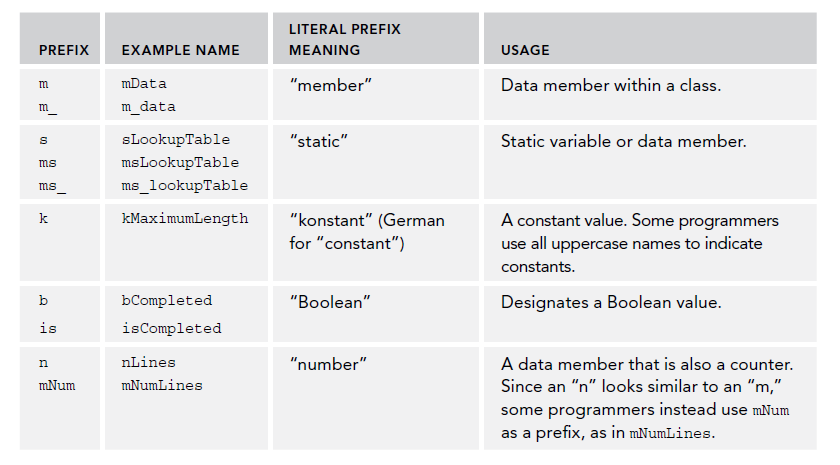
\includegraphics[scale = 0.6]{Naming.png}
				\end{figure}

			\subsubsection{使用}
			\begin{itemize}
				\item 初始化变量-值化(int, 指针, 结构体,  堆空间)
				\item 不定义多余的变量  
				\item 类的构造函数需初始化所有类成员,否则可能遗留问题
				\item 引用是某块内存的别名,不能改,且不能为空
				\item 静态成员(所有对象的值)需要初始化,且在类外进行,初始化时不需要加 访问权限,又因静态成员属于所有对象,所以初始化应指明其类名。
			\end{itemize}
		\subsection{运算符使用问题}
			\begin{itemize}
				\item 
			\end{itemize}
		\subsection{函数问题}
			\begin{itemize}
				\item 
			\end{itemize}
		\subsection{条件语句问题}
			\begin{itemize}
				\item 
			\end{itemize}
		\subsection{循环语句问题}
			\begin{itemize}
				\item 
			\end{itemize}
		\subsection{数值类型转换问题}
			\begin{itemize}
				\item 随机数 \url{http://blog.csdn.net/beyond0824/article/details/6009908}
			\end{itemize}
\section{内存管理}
		\subsection{内存分配与使用}
			\begin{itemize}
				\item 
			\end{itemize}
		\subsection{内存泄漏}
			\begin{itemize}
				\item 
			\end{itemize}
\section{缓冲区溢出}
		\subsection{数组越界}
			\begin{itemize}
				\item 
			\end{itemize}
		\subsection{数据越界}
			\begin{itemize}
				\item 
			\end{itemize}
		\subsection{字符串操作溢出}
			\begin{itemize}
				\item 
			\end{itemize}

\section{指针问题}
		\subsection{定义问题}
			\verb|#define INT_PTR int*| 这是\textbf{宏定义},编译预处理阶段要进行宏替换,\verb|INT_PTR a,b会变成 int* a,b| 所以b不是指针类型
			
			\verb|typedef int* int_ptr;| 这是\textbf{自定义类型},也就是把\verb|int_ptr|定义为 int型指针,编译阶段会把c,d\textbf{都识别}为指针
			
		\subsection{空指针解引用}
			\begin{itemize}
				\item 
			\end{itemize}
		\subsection{指针非法使用}
			\begin{itemize}
				\item 
			\end{itemize}
			
		\subsection{数组参数}
			数组做函数参数时,\textbf{当做普通指针}来用
			
\section{安全缺陷}
		\subsection{外部输入安全缺陷}
			\begin{itemize}
				\item 
			\end{itemize}
		\subsection{资源泄漏}
			\begin{itemize}
				\item 
			\end{itemize}
		\subsection{其他}
			\begin{itemize}
				\item 
			\end{itemize}
		
\section{类}
	\subsection{类命名问题}
		\begin{itemize}
			\item  \verb|类名| 首字母大写
			\item  \verb|类成员函数| 首字母小写,以驼峰样式命名
			\item  \verb|类成员变量| 遵照变量命名规则
		\end{itemize}
		
		\begin{lstlisting}
	class SpreadsheetCell
	{
	public:
		void setValue(double inValue);
		double getValue() const;
	private:
		double mValue;
	};
		\end{lstlisting}

	\subsection{访问权限}
		In C++, a struct can have methods just like a class. In fact, the only difference is that the \textbf{default
		access specifier for a struct is public} while the \textbf{default for a class is private}. For example, the
		SpreadsheetCell class can be rewritten using a struct as follows
		
		\begin{lstlisting}
	struct SpreadsheetCell
	{
		void setValue(double inValue);
		double getValue() const;
	private:
		double mValue;
	};
		\end{lstlisting}
	
	\subsection{区分对象所在处}
		\subsubsection{Object on the Stack}
			\verb|RAII|:You create objects \textbf{just as }you \textit{declare} \textbf{simple variables}, except that the variable type is the class
			name
			\begin{lstlisting}
	SpreadsheetCell myCell, anotherCell;
	myCell.setValue(6);
	anotherCell.setString("3.2");
	cout << "cell 1: " << myCell.getValue() << endl;
	cout << "cell 2: " << anotherCell.getValue() << endl;
			\end{lstlisting}
			
		\subsubsection{Object on the Heap}
			使用 \verb|new操作符| 动态的分配的空间一般都处于 堆区
		\begin{lstlisting}
	SpreadsheetCell* myCellp = new SpreadsheetCell();
	myCellp->setValue(3.7);
	delete myCellp;
	myCellp = nullptr;
		\end{lstlisting}
		
\section{其他}
		\subsection{预处理}
			\begin{itemize}
				\item 
			\end{itemize}
		\subsection{异常}
			\begin{itemize}
				\item 
			\end{itemize}
		\subsection{多线程和同步性}
			\begin{itemize}
				\item 
			\end{itemize}
		\subsection{代码不可达}
			\begin{itemize}
				\item 
			\end{itemize}
		\subsection{关于VS2013中的相对路径问题}
			\begin{itemize}
				\item  项目开发的时候,相对路径是以project.vcproj为起点
				\item  分隔符使用“//”
			\end{itemize}	
		\subsection{编译}
			\begin{itemize}
				\item  LNK2001,2005: \url{http://www.mamicode.com/info-detail-1149828.html}
				\item  warning C4018: “<”:有符号/无符号不匹配[detecot.size() 在容器说明中 被定义为: unsigned int 类型, 而j是int 类型 所以会出现: 有符号/无符号不匹配警告] \url{http://blog.csdn.net/huang\_xw/article/details/8456157}
				
				\item  warning C4316: ... : object allocated on the heap may not be aligned 16
				
				\url{http://stackoverflow.com/questions/20104815/warning-c4316-object-allocated-on-the-heap-may-not-be-aligned-16}
				
				\item LNK1120: 10 个无法解析的外部命令 :\url{http://bbs.csdn.net/topics/390962489}
				
				\item LNK2019: 无法解析的外部符号 \_\_imp\_\_InitCommonControlsEx@4,该符号在函数 \_WinMainN@16 中被引用 
				
				\textbf{项目、属性、链接器、输入、附加依赖项:填写附加依赖库的名字.lib 空格或分号间隔多项}
			\end{itemize}
\end{document} 
 		    